\documentclass{mimosis}

\usepackage{needspace}

\usepackage{metalogo}
\usepackage[super]{nth}
\usepackage{amssymb}
\usepackage{amsmath}
\usepackage{amsfonts}
\usepackage{mathtools}
\usepackage{ebproof}
\usepackage{stmaryrd}

\usepackage{makecell}
\usepackage{tcolorbox}
\usepackage{xcolor}
\usepackage[pdf]{graphviz}

\usepackage{footnote}
\makesavenoteenv{tabular}

\usepackage{tikz}
\usetikzlibrary{shapes.geometric, arrows, quotes}
\usepackage{pgfplots}
\pgfplotsset{compat=1.18}

%TC:envir table 0 1
%TC:envir table* 0 1
%TC:envir tabular [ignore] word
%TC:envir displaymath 0 word
%TC:envir math 0 word
%TC:envir comment 0 0
%TC:macro \texttt [ignore]
%TC:macro \mintinline [ignore]
%TC:macro \cite [ignore]
%TC:macro \textcite [ignore]

\newcommand{\todoaround}{\begin{center} \textcolor{purple}{TODO} \end{center}}
\newcommand{\todohere}{\textcolor{purple}{TODO}}
\newcommand{\todoaroundof}[1]{\begin{center} \textcolor{purple}{TODO: {#1}} \end{center}}
\newcommand{\todohereof}[1]{\textcolor{purple}{(TODO: {#1})}}

%%%%%%%%%%%%%%%%%%%%%%%%%%%%%%%%%%%%%%%%%%%%%%%%%%%%%%%%%%%%%%%%%%%%%%%%
% Adjustments
%%%%%%%%%%%%%%%%%%%%%%%%%%%%%%%%%%%%%%%%%%%%%%%%%%%%%%%%%%%%%%%%%%%%%%%%

\usepackage{etoolbox}

% Centred minted environment
\usepackage{xpatch,letltxmacro}
\LetLtxMacro{\cminted}{\minted}
\let\endcminted\endminted
\xpretocmd{\cminted}{\RecustomVerbatimEnvironment{Verbatim}{BVerbatim}{}}{}{}

%TC:envir minted [ignore] ignore
%TC:envir cminted [ignore] ignore

%%%%%%%%%%%%%%%%%%%%%%%%%%%%%%%%%%%%%%%%%%%%%%%%%%%%%%%%%%%%%%%%%%%%%%%%
% Hyperlinks & bookmarks
%%%%%%%%%%%%%%%%%%%%%%%%%%%%%%%%%%%%%%%%%%%%%%%%%%%%%%%%%%%%%%%%%%%%%%%%

\usepackage[%
  colorlinks = true,
  citecolor  = RoyalBlue,
  linkcolor  = RoyalBlue,
  urlcolor   = RoyalBlue,
  unicode,
  ]{hyperref}

\usepackage{bookmark}

%%%%%%%%%%%%%%%%%%%%%%%%%%%%%%%%%%%%%%%%%%%%%%%%%%%%%%%%%%%%%%%%%%%%%%%%
% Bibliography
%%%%%%%%%%%%%%%%%%%%%%%%%%%%%%%%%%%%%%%%%%%%%%%%%%%%%%%%%%%%%%%%%%%%%%%%
%
% I like the bibliography to be extremely plain, showing only a numeric
% identifier and citing everything in simple brackets. The first names,
% if present, will be initialized. DOIs and URLs will be preserved.

\usepackage[%
  autocite     = plain,
  backend      = biber,
  doi          = true,
  url          = true,
  giveninits   = true,
  hyperref     = true,
  maxbibnames  = 99,
  maxcitenames = 1,
  sortcites    = true,
  style        = numeric,
  ]{biblatex}

\input{bibliography-mimosis}
\addbibresource{Thesis.bib}
% \addbibresource{Proposal.bib}  % FIXME

%%%%%%%%%%%%%%%%%%%%%%%%%%%%%%%%%%%%%%%%%%%%%%%%%%%%%%%%%%%%%%%%%%%%%%%%
% Fonts
%%%%%%%%%%%%%%%%%%%%%%%%%%%%%%%%%%%%%%%%%%%%%%%%%%%%%%%%%%%%%%%%%%%%%%%%

\ifxetexorluatex
  \usepackage{unicode-math}
  \setmainfont{EB Garamond}
  \setmathfont{Garamond Math}
  \setmonofont[Scale=MatchLowercase]{Source Code Pro}
\else
  \usepackage[lf]{ebgaramond}
  \usepackage[oldstyle,scale=0.7]{sourcecodepro}
  \singlespacing
\fi


%%%%%%%%%%%%%%%%%%%%%%%%%%%%%%%%%%%%%%%%%%%%%%%%%%%%%%%%%%%%%%%%%%%%%%%%
% Index & Glossary
%%%%%%%%%%%%%%%%%%%%%%%%%%%%%%%%%%%%%%%%%%%%%%%%%%%%%%%%%%%%%%%%%%%%%%%%


\newacronym[description={Common subexpression elimination}]{CSE}{CSE}{common subexpression elimination}

\newglossaryentry{Python}{%
  name        = {Python},
  description = {A dynamically-typed interpreted language},
  sort        = {Python},
}

\newglossaryentry{NumPy}{%
  name        = {NumPy},
  description = {Python library implementing efficient operations on multidimensional arrays},
  sort        = {NumPy},
}

% \makeindex
% \makeglossaries

%%%%%%%%%%%%%%%%%%%%%%%%%%%%%%%%%%%%%%%%%%%%%%%%%%%%%%%%%%%%%%%%%%%%%%%%
% Incipit
%%%%%%%%%%%%%%%%%%%%%%%%%%%%%%%%%%%%%%%%%%%%%%%%%%%%%%%%%%%%%%%%%%%%%%%%

\title{Embedding Pointful Array Programming in~Python}
\subtitle{Points for Free}
\author{Jakub Bachurski}

\begin{document}

%TC:ignore
\frontmatter
\renewcommand*{\thefootnote}{\fnsymbol{footnote}}
  \begin{titlepage}
  \vspace*{5cm}
  \makeatletter
  \begin{center}
    \begin{Huge}
      \@title
    \end{Huge}\\[0.1cm]
    %
    \begin{Large}
      \@subtitle
    \end{Large}

    \emph{by}\\
    \@author
    %
    \vfill
    % A document submitted in partial fulfillment
    % of the requirements for the degree of\\
    % \emph{Bachelor of Arts}\\
    % at the\\
    % \textsc{University of Cambridge}
  \end{center}
  \makeatother
\end{titlepage}

% \newpage
% \null
% \thispagestyle{empty}
\newpage

  \section*{Declaration of originality}

I, Jakub Bachurski of Trinity College, being a candidate for Part II of the Computer Science Tripos, hereby declare that this dissertation and the work described in it are my own work, unaided except as may be specified below, and that the dissertation does not contain material that has already been used to any substantial extent for a comparable purpose. In preparation of this dissertation I did not use text from AI-assisted platforms generating natural language answers to user queries, including but not limited to ChatGPT. I~am content for my dissertation to be made available to the students and staff of the University.

\vspace{1em}
% \textit{Fragments of text from papers written in conjunction with the project -- for the ACM Student Research Competition and the 10th ARRAY Workshop -- may occur in the text of this dissertation.}

\vspace{1cm}
\begin{tabular}{ll}
    Signed & \textit{Jakub Bachurski} \\
    Date & \textit{\today}
\end{tabular}


  \section*{Proforma}
\begin{tabular}{ll}
    Candidate Number & \todohere \\ % \textbf{2405E} \\
    Title & \textbf{Embedding Pointful Array Programming in Python} \\ 
    Examination & \textbf{Computer Science Tripos -- Part II, 2024} \\
    Word Count & \todohere \\
    Code Line Count & \todohere \\
    Project Originator & The candidate \\
    Project Supervisor & Professor Alan Mycroft \\
\end{tabular}

\subsection*{Original aims of the project}
Machine learning and scientific computing ecosystems are dominated by implementations of the \textit{array programming model} in Python, such as NumPy.
Writing and maintaining programs in the model is known to be difficult.
However, significant engineering effort has been spent on making it efficient.

This project set out to investigate \textit{pointful array programming} as an alternative.
The core aim was designing and implementing a pointful array language embedded in Python. 
Furthermore, the project would explore methods to execute it with Python's established array libraries. 
Thus, it would the expressiveness of pointful array programming and performance of the array programming model.
% , thus allowing programmers to \textit{escape the pointless}.

\subsection*{Work completed}

The project was a complete success. All success criteria were met with greatly extended scope, with the designed embedded language -- Ein -- implementing various array programming features previously unavailable in Python. An efficient compilation scheme from pointful array programming to the array programming model was developed, relying on a new formal connection between the two styles. 

% Research done as part of this project
My project won \textbf{first prize} among undergradutes in the ACM Student Research Competition at the 51st POPL conference. Furthermore, a research paper coauthored with my supervisor was submitted to the 10th ARRAY Workshop and \textbf{accepted} for publication.

\subsection*{Special difficulties}
None.


  {\hypersetup{hidelinks}
  \tableofcontents}

  % \section*{Acknowledgements}
  % I am most grateful to Professor Mycroft, for being the best supervisor I could have wished for. \\
  % I would like to thank my parents for always believing in me and supporting me along my journey here.
  % \clearpage
 
\mainmatter
\setcounter{footnote}{0}
\renewcommand*{\thefootnote}{\arabic{footnote}}

%TC:endignore
  \chapter{Introduction}

In his Turing Award Lecture, \textit{Notation as a Tool of Thought}, Iverson argues for the importance of programming language design through the lens of mathematical notation  \cite{iverson2007notation}. The \textit{array programming model} he introduced in APL is still in use today thanks to its performance and conciseness. The ideas presented by it were revolutionary, particularly the brevity of the language and expressiveness despite its relatively simple grammar. It contrasts in many ways with numerical languages of its time, such as FORTRAN -- as Smillie describes in \textit{Discovering Array Languages} \cite{smillie2000lecture}. 

APL's ideas certainly stood the test of time in its various implementations and the languages it influenced, such as J or MatLab. But this begs the question -- is the model still appropriate for use in modern applications such as deep learning, or is there need for a new notation?

\section{Motivation}

When I found myself in a research team working on generalisation of deep learning models, I was shocked to see novel model architectures attract Python implementations as troublesome as \href{https://github.com/google-deepmind/clrs/blob/8697f51663bd77548f4b3108816c84d163883361/clrs/_src/processors.py#L140}{this one}, which I paraphrase below in the style of \textit{NumPy:}
% FIXME: Currently, the snippet defines logits and values, but does not use the former. Also fix in Ein.
\begin{center}
\begin{cminted}{python}
att_1 = expand_dims(att_1, axis=-1)
att_2 = expand_dims(att_2, axis=-1)
att_g = expand_dims(att_g, axis=-1)
logits = (
    transpose(att_1, (0, 2, 1, 3)) +  # + [B, H, N, 1]
    transpose(att_2, (0, 2, 3, 1)) +  # + [B, H, 1, N]
    transpose(att_e, (0, 3, 1, 2)) +  # + [B, H, N, N]
    expand_dims(att_g, axis=-1)       # + [B, H, 1, 1]
)                                     # = [B, H, N, N]
\end{cminted}
\end{center}
Problems found in this snippet are not uncommon in the domain. The code was difficult to write and is not much easier to read, there are plenty of cryptic parameters that are \textit{probably correct}, and it was necessary to add comments. These issues can be attributed to a failure of the underlying paradigm -- the array programming model. \textcite{paszke2021getting} argue why the model might not be an apt abstraction for modern workflows. Though there are certainly benefits, such as the abundant parallelism present and usually good behaviour under automatic differentiation, there are also shortcomings. In short, the notation is often too explicit while also being too unconstrained, leading to code unreadable by both humans and machines. 

Matters get worse when one realises the deep learning ecosystem is extremely centralised -- nearly all research and a significant part of engineering takes place in Python in a select few libraries. Examples include PyTorch, TensorFlow, Jax, and they turn out to all derive from the aforementioned NumPy, which embraces the array programming model. 
% Even attempts at interoperability like the ONNX standard end up using the same paradigm, preserving the status quo \cite{jin2020compiling}. 
This makes implementing high-performance compilers unexpectedly hard, leading to the introduction of different intermediate representations \cite{feng2023tensorir}, posing challenges in translation to their different paradigms. The deep learning ecosystem is also constantly evolving, with new operations and hardware targets constantly developed. This makes for a colossal engineering effort in any single array compiler project, slowing down development of new practical approaches.

\section{Prior art}

Typical examples of languages used for numeric programming include C/C++, FORTRAN, or Julia. They tend to have influences from APL (in design \cite{bernecky1991fortran} or packages \cite{eigenweb}), but are primarily performance-focused imperative languages -- which do grant higher degree of control at the expense of the need for more challenging compilation schemes to produce efficient programs \cite{grosser2012polly}. The situation is similar when programming hardware accelerators such as GPUs with the C family languages. Importantly, all of these are seldom applied in deep learning directly, and rather they are called from Python via its foreign function interface. One usually only resorts to them when the existing frameworks fail.
% C/C++ are exceptions to the rule, due to their interoperability with Python and impact on GPGPU programming -- hence much of the numerical heavy-lifting is done with them. 

Issues of the array programming model have not gone unnoticed in the Python community. Many of the problems revolve around higher-dimensional arrays, which have become commonplace in the domain. And similar to Iverson's approach, mathematical notation was sought after as a inspiration for an alternative -- in this case it was \textit{Einstein summation}. Initially limited approaches in Python -- such as \textit{Tensor Comprehensions} \cite{vasilache2018tensor} and \texttt{einops} \cite{rogozhnikov2021einops} -- can be seen as the emergence of \textbf{pointful array programming}. This paradigm -- best exemplified by the Dex language \cite{paszke2021getting} -- aims to fix many problems of the established model, taking centre stage in this project. 

\section{Aims}

The main aim of the project is to design and implement a domain-specific language that pragmatically addresses problems of the array programming model, particularly in deep learning. This meant that:
\begin{itemize}
    \item The designed language needs to show improvement of notation on a selection of problems. It should be general enough to avoid awkward code switching and build on a formal foundation. There is a tool for every problem, and so we improve on the array programming model where it falls short. 
    \item Since Python is such an important aspect of the target domain, the deliverable needs to be easily integrated with it. Attention should be paid to practicality and flexibility.
    \item Due to the significant effort needed to produce efficient array code targeting all kinds of hardware, the compiler should capitalise on existing efforts in established projects to achieve this universality.
\end{itemize}
Based on these criteria, I chose to embed a new pointful array language in Python, and to compile it to calls in the NumPy library in a fashion that is easy to generalise to similar targets. 

\paragraph{Foreshadowing} The motivating example translates to the following code in my new language:
\begin{center}
\begin{cminted}{python}
logits = array(
    lambda b, h, u, v: s[b, u, h] + t[b, v, h] + e[b, u, v, h] + g[b, h]
)
\end{cminted}
\end{center}
The code became much closer to an index-oriented mathematical notation. The cryptic transpositions are gone. Most importantly -- this alternative implementation executes just as fast as the original, while being much more readable.

  \chapter{Preparation}

\section{Array programming}

\subsection{Array programming model in NumPy}

Much of today's deep learning and scientific computing workflows takes place in the \textit{array programming model}, as introduced in APL by \textcite{iverson1962programming}. A key notion underlying this style is \textbf{whole-array operations}. The leading Python library for efficiently processing multidimensional arrays, NumPy, is no exception \cite{harris2020array}. NumPy focuses on execution on CPUs and its operations are implemented in highly-optimised C and C++, and plays a central rule in numeric programming across the entire Python ecosystem. The core data structure is the \texttt{\textbf{ndarray}} -- a multidimensional rectangular array of primitive values (e.g. floating point numbers). Throughout this work we refer to these as just \textit{arrays}. 
% Some sources use the name \textit{tensors}.

We now introduce common terms when dealing with arrays. The number of dimensions of an array is called its \textit{rank}. We call arrays of rank 0  -- scalars, rank 1 -- vectors, and rank 2 -- matrices. Rectangular arrays have a consistent size in every axis, and as such have a \textit{shape}, which is a tuple of natural numbers the same length as the rank of the array. Indexing into an array $a$ of shape $(d_1, ... d_k) \in \mathbb{N}^k$ is defined for exactly the indices $(i_1, ..., i_k) \in \mathbb{N}^k$ such that $0 \le i_p < d_p$, and is usually denoted $a[i_1, ..., i_k]$.

\begin{figure}[h]
    \centering
    $$ \begin{pmatrix}
    0 & 1 & \\
    0 & 1 & 2
    \end{pmatrix} \text{ is not a rectangular array.} $$
    $$ A = \begin{bmatrix}
        1 & 2 & 3 \\ 
        4 & 5 & 6
    \end{bmatrix} \quad \mathrm{shape}(A) = (2, 3)  \quad \mathrm{rank}(A) = \mathrm{length}\left(\mathrm{shape}(A)\right) = 2 \quad A[0, 2] = 3 $$
    \caption{Examples of array concepts}
    \label{fig:array-examples}
\end{figure}

\subsubsection{NumPy Programming} 

We now give a quick rundown of the key features of NumPy. This finds many parallels in other DSLs impacted by APL, and particularly the Python deep learning frameworks which directly derive from NumPy. Efficiency of these primitives relies on the use of \textbf{strides} \cite{harris2020array} -- we treat this as an implementation detail.

\paragraph{Broadcasting}



\paragraph{Shape manipulation}

\paragraph{Reductions}

\subsubsection{Note on jagged arrays}

\textit{Jagged} (i.e. non-rectangular) arrays are used much less often than their counterpart, as they cause irregular parallelism, which is tough to implement generally and efficiently. NumPy and similar frameworks forbid them entirely. This is not unprecedented -- the same constraint is present in other array languages such as Futhark, and type-level preservation of rectangular arrays can be seen as one of the core features of the dependent type system in Dex.

\subsection{Pointful array programming}

In functional programming, one can distinguish a \textbf{point-free} (tacit, or ``pointless'') style and contrast it with the typical \textbf{pointful} one. This distinction essentially considers whether data flow is given by variable names, or driven with combinators. A classical theoretical example is that of $\lambda$ and SKI calculi, which are respectively pointful and point-free. Both have the same expressive power, but it is known that compiling $\lambda$ to SKI \textit{(bracket abstraction)} incurs an overhead, which is dependent on the expressiveness of the combinators \cite{lachowski2018complexity}. 
In essence, one can see the main result of this work as bracket abstraction for array programs.

\begin{figure}[h]
\centering
\begin{subfigure}{.3\textwidth}
  \centering
    \begin{cminted}{haskell}
sum = foldr (+) 0
    \end{cminted}
      \caption{Point-free}
\end{subfigure}%
\begin{subfigure}{.3\textwidth}
  \centering
  \begin{cminted}{haskell}
sum [] = 0
sum (x:xs) = x + sum xs
  \end{cminted}
  \caption{Pointful}
\end{subfigure}
\caption{Point-free and pointful styles of a Haskell \texttt{sum} function}
\label{fig:point-haskell}
\end{figure}

In the context of this work we draw a similar distinction in array programming as \textcite{paszke2021getting} -- the array programming model is \textit{point-free}, because we reason on whole arrays and stylistically do not operate on individual indices. In contrast, \textit{pointful} array programming shall allow us to reason more explicitly about single elements in arrays. This pushes indexing operations to the fore-front and, at the very least, yields a stylistic 
improvement that brings us closer to \textbf{mathematical 
notation}.

\begin{figure}[h]
\centering
\begin{subfigure}{.4\textwidth}
  \centering
    \begin{cminted}{python}
c = multiply(
  transpose(a, (1, 0)),
  expand_dims(b, 1))
    \end{cminted}
      \caption{Point-free NumPy}
\end{subfigure}%
\begin{subfigure}{.4\textwidth}
  \centering
  \begin{cminted}{haskell}

c = for i j. a.j.i * b.j
  
  \end{cminted}
  \caption{Pointful Dex}
\end{subfigure}
\caption{Point-free and pointful array programs in NumPy and Dex}
\label{fig:point-arrays}
\end{figure}


\subsubsection{Einstein summation}

\subsubsection{Languages}

This section does not aim to be  \textbf{Dex} is likely the best modern example of a pointful array language. It features a value-dependent type system for keeping track of array sizes, and embraces the various parallels between arrays and functions. Its main shortcoming is its bespoke LLVM compiler and need to write binding code with other frameworks, both of which introduce friction when using it in practice.

It is worth is worth to mention the $\tilde{F}$ calculus introduced by \textcite{shaikhha2019efficient}. After extensions to the Phi calculus introduced in the proposal for this project, it was discovered that it bears close resemblance, and as such has been a major influence. However, it does not have an open implementation, and its proposed compiler relies on C code generation. Lastly, the array comprehensions of Single-Assignment~C can be seen as a precursor feature of pointful array programming \cite{scholz1994single}. Pointful DSLs often feature comprehension-like constructs, which are prevalent in modern programming languages generally (e.g. Python and Haskell). 

% \subsection{Mapping to hardware}

% \subsection{Other approaches}

% \subsubsection{Functional}

% \subsubsection{Named tensors}

% \subsubsection{Macro-based}

\section{Domain-specific languages}

The practice of creating domain-specific languages (DSLs) has a long history \cite{hudak1996building}. General programming or even properties such as Turing-completeness or fallibility are not necessary in some contexts. Carefully designing what is possible in the language improves the programming experience and simplifies compilation. 

\subsection{Embeddings}

A domain-specific language can be standalone, wherein it functions independently of the rest and uses its own syntax entirely. However, a dominant approach is \textbf{embedding} them in a host language and taking advantage of the host's syntax. Furthermore, we distinguish two kinds of embeddings: \textit{deep} (where the DSL execution manipulates the syntax tree) and \textit{shallow} (the DSL is executed directly) \cite{gibbons2014folding}. Generally, shallow-embedded languages are much easier to integrate with existing codebases and host language features. In particular, depending on the techniques used, DSL programs become values, and hence the host language programmer can apply metaprogramming techniques to transform them.

\subsubsection{Tracing}

In the context of Python, a common approach to creating shallow-embedded DSLs is \textbf{tracing}, which has found use in the novel Jax framework as described by \textcite{frostig2018compiling}. A DSL program is enclosed by a function in the host language, and to compile a program the function is \textit{traced} by calling it with placeholder (symbolic) arguments, representing the possible variable inputs. Computations are performed \textit{lazily} on these arguments -- no work is done immediately, and instead a computational graph is constructed. Once the function returns, this graph is captured and the program can be compiled and executed.
\begin{figure}[ht]
    \centering
    [Give an example of tracing here]
    \caption{Example of tracing in a Python DSL}
    \label{fig:tracing}
\end{figure}
This approach is predictable and leads to a kind of multi-stage programming, wherein before the results are determined, the entire program can first be collected and compiled. Tracing is often combined with function polymorphism (e.g. operator overloading), so that traced programs look as if they were \textit{eager}. A limitation of this approach is that runtime-dependent control flow cannot be traced directly.

\section{Functional programming patterns}

This work makes use of some patterns that are present in literature on functional programming, as well as languages such as Haskell.

\subsection{Applicative functors}

\textcite{mcbride2008applicative} introduced the notion of an \textbf{applicative functor} -- a functional programming pattern that generalises monads and specialises functors -- which is a well-behaved structure that defines certain primitive operations that behave well under composition. One of the central structures introduced in this work is an applicative, and so we introduce these operations here. We say $f$ is an applicative functor if the following operations are defined:
\begin{itemize}
    \item $\mathrm{return} : \alpha \to f\,\alpha$
    \item $\circledast : f\,(\alpha \to \beta) \to f\,\alpha \to f\,\beta $
\end{itemize}
These operations must follow the \textit{applicative laws}, which can be seen in the light of homomorphisms in a categorical sense, or just a notion of niceness under function composition. In this work we use a bijectively constructed variation of $\circledast$ (pronounced \textit{apply}), $\mathrm{lift}$:
\begin{align*}
\mathrm{lift}_2& : (\alpha \to \beta \to \gamma) \to f\,\alpha \to f\,\beta \to f\,\gamma \\ 
\mathrm{lift}_2&\,f\,a\,b = (f \circledast a) \circledast b
\end{align*}
$\mathrm{lift}$ generalises to arbitrary numbers of function arguments via an analogical construction. Applicatives can be seen as a sort of container or embellishment that allows application of transformations in the same context. Two examples of applicatives, $\mathrm{List}$ and $\mathrm{ZipList}$ are shown on Figure \ref{fig:applicatives}.
%
\begin{figure}[h]
\centering
\begin{subfigure}{.5\textwidth}
  \centering
  \begin{align*}
\mathrm{return}\,x &= [x] \\
\mathrm{lift}\,f\,a &= \mathrm{map}\,(\lambda\,(h, x) \ldotp h\,x)\,(f \times a)
  \end{align*}
  \caption{$\mathrm{List}$ (nondeterminism) applicative for arbitrary lists \\ -- pairwise application ($\times$ is the Cartesian product for lists)}
\end{subfigure}%
\begin{subfigure}{.5\textwidth}
  \centering
  \begin{align*}
\mathrm{return}\,x &= \mathrm{replicate}\,n\,x \\
\mathrm{lift}\,f\,a &= \mathrm{map}\,(\lambda\,(h, x) \ldotp h\,x)\,(\mathrm{zip}\,f\,a)
  \end{align*}
  \caption{$\mathrm{ZipList}$ applicative on lists of fixed length \\ -- respective application}
\end{subfigure}
\caption{Examples of applicatives functors}
\label{fig:applicatives}
\end{figure}

\textit{Representable} or \textit{Naperian} functors are a related notion that generalises array-like collections -- these are also useful abstraction in array programming, as shown by \textcite{gibbons2016aplicative}. However, the structure we describe later on is a bit more general, so we do not go into detail here.

\subsection{Monoids}

A \textbf{monoid} is an algebraic structure defined through an associative operation $\oplus$ (concatenation) and identity element $\varepsilon$, i.e.:
$$ (a \oplus b) \oplus c = a \oplus (b \oplus c) \quad a \oplus \varepsilon = \varepsilon \oplus a = a $$
Monoids are an extremely important abstraction in parallel programming particularly thanks to the associativity property, thanks to which computation of \textit{reductions} can be efficiently parallelised via various work partitioning patterns. A simple divide-and-conquer halving pattern could be written as:
$$ \bigoplus_{i=1}^{2n} f(i) = \bigoplus_{i=1}^{n} f(i) \oplus \bigoplus_{i=n+1}^{2n} f(i) $$

\section{Compiler techniques}

\subsection{Redundancy elimination}

\subsubsection{Common subexpression elimination}

\subsubsection{Loop-invariant code motion}

\subsection{Equivalence classes}

The analysis used in this work can be seen as a special case of the term-equality judgement used in dependently-typed systems.

\subsection{Abstract interpretation}

\section{Starting point}

\section{Requirements analysis}

\section{Software engineering}

\subsection{Methodology}

\subsection{Choice of tools}

\subsection{Review of test suites}

\subsection{Licensing}

  \chapter{Implementation}

We consider this project to be the implementation of a compiler for a domain-specific language. Throughout this chapter, we follow compiler phases from the frontend to the backend. 
\begin{itemize}
    \item We first introduce the \textit{Phi calculus}, which formalises pointful array programs (Section \ref{phi-calculus}). We consider its syntax, type system, and semantics.
    \item In Section \ref{ein-dsl} we showcase the domain-specific language itself -- \textit{\textbf{Ein}}. We describe its deep-embedding in Python. Since we use an embedding, we do not need a classical parser. Ein's API builds up expressions in Phi, after which a complete program can be explicitly \textit{evaluated}.
    \item To evaluate the program, we have to \textit{compile} it. We describe the most important analyses and transformations which form the Ein compiler's middle-end in Sections \ref{compiler-analyses} and \ref{compiler-transformations} respectively.
    \item A key contribution of this work is the novel \textit{code generation} scheme, which allows us to ``escape the pointless'' (Section \ref{escaping-the-pointless}). We define our compilation target for programs in the array programming model -- \textit{Yarr}, our point-free array calculus. The \textit{Axial} applicative functor is introduced, underlying the connection between pointful and point-free array programming in terms of Phi and Yarr.
    \item Once the program is represented in Yarr, we interpret it through an \textit{execution backend}. We primarily use NumPy, but we also show our approach is general enough to also work for an established framework like PyTorch (Section \ref{execution-backend}).
    \item We wrap up the chapter with a repository overview in Section \ref{repository-overview}.
\end{itemize}
Throughout this section code snippets are excerpts from executable Python using Ein. 


\section{Theory -- Phi calculus}
\label{phi-calculus}

We begin by introducing the functional \textbf{Phi calculus}, which is the theoretical basis for Ein. I outline the design choices I made, and how they relate to the real capabilities of array libraries.

\subsection{Grammar and design}

\newcommand{\philet}[3]{\mathrm{let}\,{#1}={#2}\,\mathrm{in}\,{#3}}
\newcommand{\phivec}[3]{\Phi\, {#1}[{#2}] \ldotp {#3}}
\newcommand{\phifold}[5]{\mathrm{fold}\,{#1}[{#2}]\,\mathrm{over}\,{#3} = {#4}\,\mathrm{by}\,{#5}}
\newcommand{\phipair}[2]{\left\langle {#1}, {#2} \right\rangle}
\newcommand{\phifst}[1]{\mathrm{fst}\,{#1}}
\newcommand{\phisnd}[1]{\mathrm{snd}\,{#1}}
\newcommand{\phisize}[2]{\mathrm{size}_{#2}\, {#1}}
\newcommand{\phiasserteq}[2]{\mathrm{assert}\,{#1}={#2}}

We define the syntax and primitives of Phi. It is largely similar to $\tilde F$, as introduced by \textcite{shaikhha2019efficient}.
\begin{align*}
e ::=&\quad \phivec{i}{e}{e} \quad|\quad e[e]   &\text{(array comprehension, indexing)} \\
|&\quad \phifold{x}{e}{x}{e}{e}  &\text{(indexed fold)} \\
|&\quad \phipair{e}{e} \quad|\quad \phifst{e} \quad|\quad \phisnd{e} &\text{(pair construction, projections)} \\
|&\quad \pi(e, \dots, e) &\text{(scalar operator)} \\
|&\quad \phiasserteq{e}{e} \quad|\quad \phisize{e}{k} &\text{(equality assertion, size along axis } k \in \mathbb N \text{)} \\
|&\quad \philet{x}{e}{e} &\text{(non-recursive let binding)} \\
|&\quad x \quad|\quad i \quad|\quad v &\text{(variable, index, constant)}
\end{align*}
The introduction form for arrays is the indexed \textit{array comprehension} $\Phi$ (pronounced \textit{for}) -- for instance, $\phivec{i}{5}{i}$ is the array $[0, 1, 2, 3, 4]$. The elimination form is \textit{indexing} $a[i]$ ($i$-th element of $a$). Phi interprets multidimensional arrays as either scalars (zero-dimensional base case) or vectors of arrays. In that respect indexing is into the \textit{outermost} axis. 

The indexed fold facilitates a simple repeated iteration with an accumulator, and is closely related to the \texttt{loop} construct in Futhark. One can see $\Phi$ as perfectly parallel, while $\mathrm{fold}$ expresses sequential computation.

Examples of scalar operators $\pi$ include arithmetic ($+$, $\times$, \dots) and logic ($\land$, $\lor$, \dots) operators. Among non-standard primitives are equality assertions, which are applied to ensure that two array dimensions have equal sizes. These sizes are obtained with the $\mathrm{size}$ primitive -- if $e$ has shape $(n, m)$, then $\phisize{e}{1} = m$.

A crucial feature of Phi is the addition of a special kind of variable -- indices $i, j, k, \dots$ -- which live in a separate namespace. They are solely introduced in array comprehensions, and receive special treatment in both the type system and the compilation scheme. We use usual variables $x, y, z, \dots$ in all other cases.

For example, the following Phi term computes the (left-associative) sum $\sum_{i=0}^{n-1} a_i$ for a vector $a$:
$$ \phifold{i}{n}{x}{0.0}{x + a[i]} $$

\subsection{Type system}

\newcommand{\phifloattype}{\mathrm{Float}}
\newcommand{\phiinttype}{\mathrm{Int}}
\newcommand{\phinattype}{\phiinttype}
\newcommand{\phibooltype}{\mathrm{Bool}}
\newcommand{\phivectype}[1]{\Box{#1}}
\newcommand{\phipairtype}[2]{{#1} \times {#2}}

The type system of Phi is relatively straightforward, except for the handling of indices. Type constructors are unconstrained, and we allow arrays of pairs (missing from most array frameworks).
\begin{align*}
\sigma &::= \phifloattype \mid \phiinttype \mid \phibooltype & \text{(scalar types)} \\
\tau &::= \sigma \mid \phivectype{\tau} \mid \phipairtype{\tau}{\tau} & \text{(Phi types -- scalars, vectors, pairs)}
\end{align*}
The typing judgement $\Gamma; \Delta \vdash e : \tau$ is slightly non-standard due to the presence of indices. We use a separate environment for variables $\Gamma$ and indices $\Delta$. Consider the rules for array comprehensions and folds:
\begin{center}
    \begin{prooftree}
        \hypo{\Gamma; \diamond \vdash n : \phinattype}
        \hypo{\Gamma; \Delta, i \vdash e : \tau}
        \infer2{\Gamma; \Delta \vdash \phivec{i}{n}{e} : \phivectype{\tau}}
    \end{prooftree} \quad
    \begin{prooftree}
        \hypo{\Gamma; \diamond \vdash n : \phinattype}
        \hypo{\Gamma; \Delta \vdash a : \tau}
        \hypo{\Gamma, k: \phinattype, x: \tau; \Delta \vdash e : \tau}
        \infer3{\Gamma; \Delta \vdash \phifold{k}{n}{x}{a}{e} : \tau}
    \end{prooftree}
\end{center}
Other typing rules are relatively standard and carry through both $\Gamma$ and $\Delta$. Note that sizes and iteration counts are typed under $\Delta = \diamond$ -- i.e. neither can depend on a comprehension index. This ensures \textit{regularity} of the parallelism involved. Since an array size cannot depend on the index at which the defined element is placed, all arrays must remain rectangular. Similarly, since all iteration counts are the same across all array elements, the same computation is applied at each index. Hence, this does not type:
$$ \phivec{i}{5}{\phivec{j}{\textcolor{red}{i}}{i + j}} $$
Regularity is a beneficial property that ensures an efficient compilation scheme. We achieve it by a simple type check, which replaces a runtime check in Futhark, or the dependent type system in Dex. 
% TODO: typing rules and semantics in appendix?

\subsection{Semantics}

\paragraph{Conditionals} Phi does not feature a dedicated conditional expression. We consider conditionals to be a ternary scalar operator instead, which we write $\mathrm{where}(c, t, f)$ (owed to the \texttt{numpy.where} primitive). As such, both branches are always evaluated regardless of the condition. This design choice follows as the array programming model has no real notion of a \textit{branching} array computation -- both cases are evaluated, as this ensures efficient vectorisation (SIMD processing). In hardware, the related notion is \textit{predication} -- particularly in GPUs or in CPU conditional move instructions.

\paragraph{Out-of-bounds} As noted, ternary conditionals evaluate both of their branches. In particular, this means that indexing operations that take place in either branch might end up out of bounds. 
The Jax framework tackles a similar problem, and in the context of hardware accelerators the best solution seems to be to gracefully recover from the error by clipping the indices or imputing a constant result. 
In Phi for simplicity we stick to clipping into bounds.

\paragraph{Invalid arguments} We consider it to be a runtime error where a size or number of iterations is negative. We do not dwell on this, as the semantics could easily be modified to be exception-free.

\subsection{Embedding Phi in Python}
\label{embedding-phi}

We embed Phi in Python to allow constructing and validating terms in the frontend. Conceptually, we implement Phi's grammar as a sum type. To implement this pattern in Python, we use a sealed abstract base class \texttt{AbstractExpr} with a child class for each case of \texttt{Expr}. To construct the term $\phivec{i}{4}{\phivec{j}{4}{i \cdot j}}$, we write:
\begin{center}
\begin{cminted}{python}
i, j = Index(), Index()
four = Const(Value(4))
table = Vec(i, four, Vec(j, four, Multiply((At(i), At(j)))))
\end{cminted}
\end{center}
Thanks to the simplicity of Phi's type system, we easily implement bottom-up type checking. To prevent the construction of invalid terms, constructors calculate a type based on the subterms. To facilitate this, we make use of intrinsically typed variables. 
Furthermore, instead of string-based variable names, we reuse their Python object identity, which is akin to using a \texttt{gensym}-like functionality.


\section{Frontend -- Ein}
\label{ein-dsl}

\textbf{Ein} forms the programmer-accessible side of the project, and is implemented as the \texttt{ein} Python package. Unlike a traditional compiler, our frontend is not formed by a lexer or parser, but \texttt{ein}'s API forming the deep-embedded DSL. We provide an overview of Ein's features and its design as a purely functional, pointful array DSL.

\subsection{Embedding}

One of the main influences on the design of the embedding is Jax \cite{frostig2018compiling}, which lays out a solid foundation.
% for encapsulating expressions and building programs up by tracing. 
% This indirection can be seen as an instance of multi-stage programming, since the constructed program can have global optimisations applied to it before execution. 
DSL values transparently encapsulate an expression type (Section \ref{embedding-phi}).
A useful feature is that let bindings in the language are implicit and later recovered by the compiler.
% object identity is used to establish the same expression is reused, which can be seen as a safe approximation of \textit{hash consing}. 
For example, say \texttt{a} is an Ein value, in which case \texttt{a + a} indicates adding \texttt{a} to itself. 
Then \texttt{a} is reused in the compiled program rather than recomputed.

\subsection{Arrays}

% All Ein values 
% Nearly all operations in Ein take place on values of the \texttt{Array} type. These incrementally construct expressions in the underlying calculus via tracing. 
Similarly to Phi, Ein considers arrays to be defined recursively as either \textbf{scalars} or \textbf{vectors} of arrays. These correspond to the \texttt{Scalar} and \texttt{Vec[T]} classes. The methods of \texttt{Scalar} correspond to the scalar operators of Phi. These can be performed with operator overloading (as in \texttt{Scalar.\_\_mul\_\_} -- \texttt{a * b}) and methods (\texttt{Scalar.sin} -- \texttt{a.sin()}). On the other hand, \texttt{Vec} implements \texttt{Vec.\_\_getitem\_\_}, so that we can write \texttt{a[i]}. These are exemplified below, with type annotations added for clarity:
\begin{center}
\begin{cminted}{python}
a: Vec[Scalar]
b: Scalar = a[0].sin() * a[1].cos()
\end{cminted}
\end{center}
Both \texttt{Scalar} and \texttt{Vec[T]} have an \texttt{expr} attribute, and succeeding values have theirs lazily built up their corresponding Phi expression. For example: 
\begin{center}
\begin{cminted}{python}
b.expr == Mul(
    Sin(Get(a.expr, const(0))), 
    Cos(Get(a.expr, const(1)))
)
\end{cminted}
\end{center}

\subsection{Combinators}

The central part of Ein are the pointful, comprehension-style \textit{combinators}: \texttt{array} and \texttt{fold}. Anonymous functions, defined with the \mintinline{python}{lambda} keyword, are applied to facilitate introduction of new variables -- for instance, the index in an array comprehension. As such, \mintinline{python}{array(lambda i: i, size=5)} describes the Phi expression $\phivec{i}{5}{i}$. Further, the summation in $\philet{a}{\phivec{i}{5}{i^2}}{ \sum_{i=0}^{4} a[i]}$ is expressed with a \texttt{fold}:
\begin{center}
\begin{cminted}{python}
a = array(lambda i: i*i, size=5)
s = fold(0, lambda i, acc: acc + a[i])
\end{cminted}
\end{center}
We avoid explicit variable introductions by making use of the host language's lambda functions, in a manner similar to \textcite{atkey2009unembedding} and Jax. The explicit approach is taken surprisingly often for the drawbacks it has -- for instance in the SymPy algebra library or Taco. In the latter we have to write:
\begin{center}
\begin{cminted}{python}
i, j = pytaco.get_index_vars(2)  # explicit introduction
S[i, j] = A[i, j] + A[j, i]      # i, j still live afterwards. danger!
\end{cminted}
\end{center}
This is evidently flawed, as there is nothing guarding against the reuse of variables in the wrong scope. 

We have noted NumPy is a first-order interface, as its operations cannot be parameterised by functions. On the other hand, \texttt{array} and \texttt{fold} are closer to Second-Order Array Combinators, which are indispensable in Futhark. They are a major step up in Ein's expressive power.



\subsection{Size inference}

% TODO: This is sort of metaprogramming.
\textit{Size inference} allows omitting the size of arrays in some contexts. Consider the following computation:
\begin{center} 
\begin{cminted}{python}
array(lambda i: a[i] + b[i], size=a.size(axis=0))
\end{cminted} 
\end{center}
Say that the vectors $\texttt{a}$ and $\texttt{b}$ have the same size. Then with size inference we may omit the explicit \texttt{size}:
\begin{center} 
\begin{cminted}{python}
array(lambda i: a[i] + b[i])
\end{cminted} 
\end{center}
Specifically, for any index \texttt{i} that does not have an explicit \texttt{size} defined, it is inferred by taking the size of any array \texttt{a} that is indexed directly with \texttt{i} (i.e. in an expression \texttt{a[i]}), which we find by term graph traversal. Where there are other such candidates \texttt{b}, we add a program assertion that \texttt{a} and \texttt{b} have the same size. We further generalise this to the \texttt{fold} combinator, as its loop counter is often used to iterate over arrays.

% This is not as obvious to implement correctly as it seems at first sight. Due to the Phi typing rules, any sizes cannot (even indirectly) depend on a comprehension index nor on a value from an inner scope. Various simplifications and checks are performed to avoid bad candidates for an inferred array size.

There are many mechanisms similar to size inference, for instance in Single-Assignment C and in a more structured way in Dex via its value-dependent type inference. 
% In DSLs taking direct inspiration from Einstein summation, such approaches are often the only way of specifying array sizes. Ein also provides the flexibility of providing an explicit array size, as shown in the former example.

\subsection{Records}

So far, we have not yet described how Ein makes use of Phi's pair types. Indeed, in Ein we use them internally for representing labelled record types. We use a basic list-like encoding, where $\{ x: \phiinttype, y: \phiinttype, z: \phiinttype \}$ becomes $\phipairtype{\phiinttype}{\left( \phiinttype \times \phiinttype \right)}$. However, in contrast to \texttt{Vec} and \texttt{Scalar}, we do not use a custom Ein class for representing records. Instead, we use builtin Python container types:
%We then directly use standard Python container types to represent Ein record values, and in fact arrays can contain these types as elements. We can write:
\begin{center} 
\begin{cminted}{python}
# Array of dictionaries (records {x: int, y: int, z: int})
a = array(lambda i: {"x": i, "y": i*i, "z": i*i*i}, size=10)
# Indexing into a returns a dictionary with the same keys (record fields)
assert list(a[4].keys()) == ["x", "y", "z"]
# a[4] -> {"x": <4>, "y": <4*4>, ...}
assert a[4]["y"].eval() == 16
\end{cminted}
\end{center}
In fact, arbitrary \textit{layouts} consisting of Python tuples, dictionaries, and dataclasses can be used as array elements -- and these are reconstructed when indexing into these arrays. This feature relies on the layouts being \textit{static}. The only dynamically-sized values are arrays, which are handled through the \texttt{Vec} class. 

This feature enables a new style of array programming, unavailable in existing libraries. It is possible to describe composable array structures of custom data types and define operations on them. For instance, one could define an array of dual numbers\footnote{Dual numbers are similar to complex numbers, but instead of the imaginary unit $i^2 = -1$ we instead have a symbol $\varepsilon^2 = 0$. They are particularly useful in forward-mode automatic differentiation, and one could use them for this purpose in Ein.} by using a dataclass:
\begin{center}
\begin{cminted}{python}
@dataclass
class Dual:
    real: Float
    eps: Float
    def __mul__(self, other: 'Dual') -> 'Dual':
        return Dual(
            self.real * other.real, 
            self.real * other.eps + self.eps * other.real
        )

a = array(lambda i: Dual(i, 1.), size=5)  # constructs Vec[Dual]
b = array(lambda i: a[i] * a[i])  # calls Dual.__mul__
\end{cminted}
\end{center}
In contrast, most renditions of the array programming model struggle to achieve this sort of composability. Since they consider \textit{whole arrays of primitives}, in Python at best one could sub-class an array, but this would not compose as well. In a pointful paradigm where we focus on individual elements, we can neatly define datatypes and consider arrays of them (like in Futhark). What is more, efficient representation of these structures is ensured via program transformations. Record types in Ein are a \textbf{zero-cost abstraction}.

\subsection{Type system}

We can now summarise the crux of Ein's \textit{type system}:
\begin{align*}
\texttt{T} \quad::=&\quad 
\text{\mintinline{python}{Scalar}}
& \text{(scalars -- atoms)} \\
\mid&\quad
\text{\mintinline{python}{Vec}}[\texttt{T}]
& \text{(vectors)} \\
\mid&\quad
\text{\mintinline{python}{dict}}[\text{\mintinline{python}{str}}, \texttt{T}] \,\mid\, \text{\mintinline{python}{tuple}}[\texttt{T}, \dots] \,\mid\, \texttt{Dataclass}_\texttt{T}
& \text{(records)}
\end{align*}
While only \texttt{Scalar} and \texttt{Vec} are classes implemented by Ein, the types $\texttt{T}$ can be used in Ein's primitives and are closed under them. We also do some implicit casting (e.g. \mintinline{python}{float} into \texttt{Scalar}).

The part of the Python object specifying record fields is called the \textit{layout}. Example layouts include the list of dictionary keys or the size of a tuple.
These layouts can be easily stored and reconstructed in Ein thanks to Python's dynamism.\footnote{As noted before, we assume the record types are static -- e.g. constant across fold iterations. This further means we take dictionaries, tuples and dataclasses to be immutable, which is part of Ein's contract.}

\subsection{Type annotations}

Ein classes are usable as Python type annotations. 
% For this purpose, we further split \texttt{Scalar} into \texttt{Int}, \texttt{Float} and \texttt{Bool}, which correspond to base types $\sigma$ in Phi. 
For instance, \mintinline{python}{a: Vec[Vec[Float]]} indicates \texttt{a} is an Ein matrix of floats. Thanks to this design, it is possible to use standard type checkers like \texttt{mypy} for \textbf{gradual typing} of Python programs using Ein. Some type errors -- like attempting to add a scalar and a vector, or indexing into a scalar -- may be discovered before runtime. Furthermore, type hints for records work on the same principle -- we previously wrote \mintinline{python}{Vec[Dual]} for a vector of dual numbers. Indexing into such a vector returns a \mintinline{python}{d: Dual}, which is known to have the fields \mintinline{python}{d.real: Float} and \mintinline{python}{d.eps: Float}.

This is a significant advancement over NumPy, where this sort of static type checking combined with user-defined data types is virtually impossible.
% TODO: Eval - composable approach leads to better behaviour under typing

% Furthermore, during tracing Ein performs a form of basic type inference on the underlying Phi expressions. Any type errors found at that stage are reported at runtime, ensuring type safety of programs produced by the compiler. 


\section{Analyses}
\label{compiler-analyses}

We now describe the main analyses applied on Phi calculus, which facilitate further transformations and efficient code generation. Since Ein produces Phi term graphs, this is the main form on which we operate.

\subsection{Normalisation of high-level operations}

\todothis

% \begin{center}
%     \textcolor{red}{Not happy with how this looks right now. The notation is really messy, and the concept of what is opaque and what is in the normal form is left unclear.}
% \end{center}

% \textit{Declarative syntax matching on summation, minimisation, etc. defined by folds, which allows us to infer what high-level operations are applied (e.g. reductions). Similarly special indexing patterns; and tensor contractions -- matrix multiplication generalised to more dimensions.} \todothis

% A particular feature of our compilation setting is that both the source and target languages are relatively high-level. Furthermore, the compilation target (NumPy, in the array programming model) has many primitives that perform specific high-level operations. Therefore, to obtain fast array code, we need to recover some of these specialised operations.

% A naive approach would be to simply match on the syntax of the operations we perform. However, this would be a volatile approach, as small changes to the source code might result in the optimisation no longer being applied. We instead use a technique similar to \textit{normalisation by evaluation} (NbE). For each expression, we consider the normal form of its subexpressions. Then we compose these normal forms by appealing to the denotational semantics of Phi.

% \paragraph{Reductions} Recall that NumPy only offers reductions for some operations. This is part of the reason why they are not directly integrated in Phi. Still, the compiler should be able generate:
% $$ \phifold{i}{n}{x}{0.0}{x + a[i]} \leadsto \texttt{numpy.sum}(\texttt{a}) $$
% For this simple case, we just match on the Phi syntax, but we allow any initial value for the accumulator. We use the normal form:
% $$ \left\llbracket \phifold{i}{n}{x}{e}{x + f(i)} \right\rrbracket = e + \mathrm{sum}( \underline{\phivec{i}{n}{f(i)}} ) $$
% We will use $\underline{e}$ to denote \textit{opaque} terms in Phi when they are a part of the normal form.

% \paragraph{Clipped shifts} Suppose that we want to compute the difference array $d$ of $a$, given by: 
% $$ d = \phivec{i}{n}{a[\min(i + 1, n - 1)] - a[i]} $$ 
% To express this in NumPy we need to use whole-array operations. Say we first compute the left hand side operand. We need to make use of \textbf{slicing} (taking subarrays) and \textbf{padding} as follows:
% \begin{center}
% \begin{cminted}{python}
% numpy.pad(
%   a[1:],      # slice starting at 1
%   (0, 1),     # pad 1 at end
%   mode='edge' # use end value for pad
% )
% \end{cminted}
% \end{center}
% We argue that such a pattern can be expressed in Phi in general with:\footnote{This does not take into account different step sizes possible in slicing. This interacts with padding in unexpected ways, and further complicates the algebra, so we leave it out.}
% $$ a[\min(\max(i + s, l), h)] $$
% Where the terms $s, l, h$ do not have any free Phi indices, and $i$ is an index which is not free in $a$. Intuitively, this patterns shifts the index $i$ by $s$, and then clips it in the range $\left[ l, h \right]$.

% We first describe the normal forms for $i + s$:
% \begin{align*}
% i &= i + \underline{0} \\
% \underline{s'} + (i + \underline{s}) &= (i + \underline{s}) + \underline{s'} = i + \underline{s + s'} \\
% \end{align*}
% We can then build up the normal forms for $\min(\max(i + s, l), h)$:
% \begin{align*}
% i + \underline{s} &= \min(\max(i + \underline{s}, -\infty), +\infty) \\ 
% \min(\min(\max(i + \underline{s}, \underline{l}), \underline{h}), \underline{h'}) &= \min(\max(i + \underline{s}, \underline{l}), \underline{\min(h, h')}) \\ 
% \max(\min(\max(i + \underline{s}, \underline{l}), \underline{h}), \underline{l'}) &= \min(\max(i + \underline{s}, \underline{\max(l, l')}), \underline{\max(h, l')})
% \end{align*}
% Where an index has a clipped-shift normal form, an appropriate slice and pad can be synthesised. 

\paragraph{Generalised tensor contractions}

\todothis

\subsection{Size equivalences}

\textit{Using equality assertions to create an equivalence judgement between sizes. Used for determining safety to elide some indexing operations and that operations do not explode memory usage.} \todothis 


\section{Transformations}
\label{compiler-transformations}

\subsection{Outlining}

The term graph form produced by Ein is particularly useful when performing analyses, as not as much information has to be carried through in contexts. However, it is not an intermediate representation apt for generating executable code. It lacks information on where values used multiple times should be stored and when should they be computed. To address this, we want to convert our \textbf{term graph} into an \textbf{abstract syntax tree}. We refer to this process as \textit{outlining}. The goal is inserting appropriate let bindings in a semantic-preserving fashion, while preventing recomputation of expressions many times. Notably, \textit{inlining} (which is also used) corresponds to removal of the let bindings inserted by outlining. We perform it simply by directly substituting all bindings, returning the AST to the term graph form.

The two main techniques applied are \textbf{common subexpression elimination} and \textbf{loop-invariant code motion}. The former rewrites computations like $e + e$ (for a \textit{non-atomic} expression $e$) to  $\philet{x}{e}{x + x}$. Meanwhile, the loop-invariant motion ensures that terms constant across loop iterations are computed before the loop. For instance, if we want to perform the following rewrite:
$$ 
\phivec{i}{n}{a[i] + \left( \phivec{j}{n}{2 \cdot b[j]} \right)[i]} \quad\leadsto\quad \philet{c}{\phivec{i}{n}{2 \cdot b[i]}}{\phivec{i}{n}{a[i] + c[i]}} 
$$
We consider both of these transformations to be a special cases of \textbf{let insertion}. As such, the implementation determines the expressions which should be let-bound and at which program point this should happen. For simplicity, we associate program points with nodes in the term graph -- which are just terms. We have reduced the problem to determining for each term $t$, a list of terms $t'$ bound at $t$, meaning we rewrite $t \leadsto \philet{x}{t'}{\{x/t'\}t}$. The substitution $\{x/t'\}$ of a variable $x$ for $t'$ is performed by syntactic replacement.

An important simplification of the problem setup is that Phi calculus is entirely pure (there are no side effects). Any let insertions performed in this manner of ``reverse-substitution'' preserve program semantics. Additionally, we make use of the assumption that all subexpressions are evaluated at least once. Recall that conditionals in Phi evaluate both conditional branches. We similarly assume all loops iterate at least once.

\paragraph{Common subexpression elimination} We perform CSE via a standard method on term graphs, which is by application of \textbf{dominators}. Consider a graph in which there is an edge $t \to t'$ whenever $t'$ is a direct subterm of $t$. Then consider the immediate dominator $t^*$ of a term $t$. By definition, we learn that $t^*$ is the smallest term that contains all instances of $t$ as a subterm. This indicates that we should let-bind $t$ at $t^*$. We perform this let-insertion for every non-atomic term $t$ for which $\mathrm{indeg}\,t > 1$. This common subexpression elimination produces an abstract syntax tree given any term graph.

We compute the immediate dominators with the \texttt{networkx} package, which has $O(n^2)$ time complexity in the worst-case. An implementation for directed acyclic graphs could be optimised to $O(n \log n)$.

\paragraph{Loop-invariant code motion} We tackle the problem of recomputing values invariant across loop iterations. We want to compute these prior to the loop. We consider \textit{loop terms} to be $\Phi$ and $\mathrm{fold}$. 

Since after CSE we have an AST, we can perform a tree traversal on it. For each term $t$, there is a stack of loop terms that it is a subterm of, and we can update it as part of the traversal. Each of these loop terms $s_\ell$ (and any let-bindings inside) introduces a set of symbols $S_\ell$, so the stack induces a sequence $(S_1, S_2, \dots, S_k)$. Denote the free symbols in $t$ as $T$. We observe the following: if $\left( S_\ell \cup \cdots \cup S_k \right) \cap T = \emptyset$, then it is safe to let-bind $t$ prior to the loop $s_\ell$. On the other hand, $t$ will be computed the fewest times if it is moved to the outermost loop. Hence, we pick the minimum $\ell$ that preserves lexical scopes. We find and insert this let-binding for all non-atomic terms $t$.

A particularly tricky part of the implementation is the ordering in which these insertions are performed. Making the wrong choices results in scope errors or infinite terms. 
% However, a careful implementation avoids these issues. 
Lastly, there are cases in which bindings may become trivial, i.e. of the form $\philet{x}{y}{e}$. To erase these, we perform a basic form of \textbf{copy propagation} by inlining (substituting) all trivial bindings.

\subsection{Array-of-structs to struct-of-arrays}

A standard technique in array programming is the array of structs (AoS) to struct of arrays (SoA) transformation. The Ein compiler uses it to reduce away the arbitray vector types to simple arrays of primitive types. This is important, as our compilation target -- NumPy,\footnote{Technically, NumPy does allow defining custom \texttt{dtype}s, but this feature is limited in use and intended for (de)serialising binary data. Corresponding features are not available in deep learning frameworks, so relying on this is undesirable.} and array libraries generally -- lack support for arrays of composite types like pairs. Once we eliminate arrays of pairs, the only types $\tau'$ are given by:
\begin{align*}
\alpha &::= \sigma \mid \Box \alpha \\
\tau' &::= \alpha \mid \tau' \times \tau'
\end{align*}
Hence, $\tau'$ can only be tuples of arrays. This vastly simplifies compilation and runtime value representation. An AoS-to-SoA transformation is also applied in $\tilde F$ and Futhark, but it is not described in detail \cite{henriksen2017futhark, shaikhha2019efficient}. 

The isomorphism the operation relies on is $\Box (\tau_1 \times \tau_2) \cong \Box \tau_1 \times \Box \tau_2$, i.e. for each array of pairs there is an equivalent pair of arrays (of the same size). As such, we need only consider the introduction and elimination forms of arrays of pairs. The core transformation is depicted in Figure \ref{fig:aos-to-soa}.

\newcommand{\phisoa}[1]{\mathcal S \left\llbracket {#1} \right\rrbracket}
\newcommand{\phitupleindex}[2]{\mathcal P \left\llbracket {#1}, {#2} \right\rrbracket}

\begin{figure}[h]
    \centering
    \begin{align*}
\phisoa {\phivec{i}{e_n}{e}}
&= \phipair{\phivec{i'}{\phisoa{e_n}}{\phifst{\phisoa{e}}}}{\phivec{i''}{\phisoa{e_n}}{\phisnd{\phisoa{e}}}}
&\text{(where }\Gamma; \Delta, i \vdash e : \phipairtype{\tau_1}{\tau_2} \text{)} \\[0.5em]
\phitupleindex{e}{e'}
&= \phipair{\phitupleindex{\phifst{e}}{e'}}{\phitupleindex{\phisnd{e}}{e'}}
&\text{(where }\Gamma; \Delta \vdash e : \phipairtype{\tau_1}{\tau_2} \text{)} \\
\phitupleindex{e}{e'}
&= e\left[ e' \right]
&\text{(where }\Gamma; \Delta \vdash e : \phivectype{\tau} \text{)} \\
\phisoa{e[e']}
&= \phitupleindex{\phisoa{e}}{\phisoa{e'}}
&\text{(where }\Gamma; \Delta \vdash e : \phivectype{\tau} \text{)} \\[0.5em]
\phisoa{e + e'}
&= \phisoa{e} + \phisoa{e'}
&\text{(and similarly for other cases)} \\[0.5em]
\phisoa{\phivectype{(\phipairtype{\tau_1}{\tau_2}})} &= \phipairtype{\phivectype{\tau_1}}{\phivectype{\tau_2}} &\text{(identity otherwise)}
    \end{align*}
    \caption{The core of the type-driven AoS-to-SoA transformation on Phi, denoted by $\mathcal S$. $\mathcal P$ maps an indexing to all arrays in the tuple. Environments $\Gamma; \Delta$ are passed through implicitly, in accordance with typing rules.}
    \label{fig:aos-to-soa}
\end{figure}

\section{Code generation -- Escaping the Pointless}
\label{escaping-the-pointless}

We now finally talk about how we can make the step from the pointful Phi calculus into the point-free array programming model. In order to create an extra layer of abstraction, we devise \textit{Yarr} (a point-free array calculus), which is the final program representation we interpret at runtime. Afterwards, we give a novel connection between pointful and point-free array programming. This is achieved through the \textit{Axial} applicative functor. We show how programs are compiled by \textit{lifting} them into the Axial.

\subsection{Compilation target -- Yarr, the array calculus}

% \textit{We first formalise our compilation target for Phi, since so far it has only been vaguely described as the API of the NumPy library.} \todothis

We use a relatively straightforward formalisation of point-free array programs, which abstracts the interface of NumPy:
\begin{align*}
e ::=&\quad \mathrm{range}(e)   &\text{(iota -- sequence of }\mathbb N\text{ from }0\text{)} \\
\mid&\quad \mathrm{transpose}(e, (n, \dots)) &\text{(permute axes)} \\ 
\mid&\quad \mathrm{squeeze}(e, (n, \dots)) &\text{(remove 1-dimensions)} \\
\mid&\quad \mathrm{unsqueeze}(e, (n, \dots)) &\text{(add 1-dimensions)} \\
\mid&\quad \mathrm{repeat}(e, e, n) &\text{(repeat array along axis)} \\
\mid&\quad \mathrm{gather}(e, e, n) &\text{(indexing along axis }n \in \mathbb N\text{)} \\ 
\mid&\quad \mathrm{elementwise}_u(e, \dots, e) &\text{(elementwise op. }u\text{)} \\
\mid&\quad \langle e, \dots \rangle \quad\mid\quad \pi_i(e) &\text{(tuples and projections)} \\
\mid&\quad \philet{x}{e}{e} &\text{(non-recursive let binding)} \\
\mid&\quad \phifold{x}{e}{x}{e}{e} &\text{(indexed fold)} \\
\mid&\quad x \quad\mid\quad v  &\text{(variables, constants)}
\end{align*}
This is the basic formulation into which we can compile Phi. It is extended with reductions $\mathrm{reduce}_u(e, n)$ along an axis, specialised indexing operations (taking, slicing), padding, and linear algebra primitives (in the form of generalised Einstein summation).

This abstraction strives to provide an interface through which various execution backends can be implemented. Note that the only significant common part with Phi is the indexed fold. In particular, indices $i$ from array comprehensions are erased entirely. In fact, the compilation scheme guarantees that no array comprehension $\Phi$ results in a $\mathrm{fold}$. Otherwise, compiling Phi would be much easier.

\subsection{Axials}

\textbf{Axials} are the key research contribution of this work. They form a novel connection between pointful and point-free array programming. Their structure is natural, in the sense that it forms an applicative functor.

\begin{center}
    \textcolor{red}{This section is rather waffly, and I'm not sure it achieves everything it should despite talking much. The compilation scheme description is of course missing, problem being that it actually does not use exactly the same axials as the part preceding it.}
\end{center}


\paragraph{Motivation}

To motivate the introduction of axials, we appeal to the separation of variables in Phi. Indeed, we take indices $i$ to be separate from the usual variables $x$. Hence, there is a similar separation of the environment $\mathrm{Env} \equiv (\mathrm{Var} + \mathrm{Index}) \to \mathrm{Value}$:
$$ \mathrm{Env} \simeq \mathrm{VarEnv} \times \mathrm{IndexEnv} $$
We use $A \simeq B$ to denote an isomorphism, where there exist a bijection between values of type $A$ and $B$. Let us now consider the denotation of a Phi expression $e$, given by $\llbracket e \rrbracket : \mathrm{Env} \to \mathrm{Value}$. This time, we can apply the currying isomorphism:
$$\llbracket e \rrbracket : \mathrm{Env} \to \mathrm{Value} \simeq \mathrm{VarEnv} \times \mathrm{IndexEnv} \to \mathrm{Value} \simeq \mathrm{VarEnv} \to (\mathrm{IndexEnv} \to \mathrm{Value})$$
We bring close attention to the structure of $\mathrm{IndexEnv} \to \mathrm{Value}$. Since indices are only introduced in array comprehensions, we know their values must range over a range of natural numbers of the form $i \in \left[ 0, n_i \right)$. We denote $n_i$ as the size of the range of an index $i$, as introduced in $\phivec{i}{n_i}{e}$. Indeed, this leads us to say that the domain of $\mathrm{IndexEnv}$ is of the form:
$$ \mathrm{dom}\,\mathrm{IndexEnv} \simeq \left[0, n_i \right) \times \left[0, n_j \right) \times \left[0, n_k \right) \times \dots $$ 
where $\iota = \{i, j, k, \dots \}$ are the free indices in $e$. But this gives a whole lot of structure to $\mathrm{IndexEnv}$. Indeed, the \textit{index space} directly corresponds to that of a $\iota$-dimensional array of shape $(n_i, n_j, n_k, \dots)$. Let us denote $\mathrm{Array}_d$ as the type of $d$-dimensional homogeneous arrays. We have the following connection:
$$ \mathrm{IndexEnv} \to \mathrm{Value} \simeq [\iota] \to \mathrm{Array}_{|\iota|}\, \mathrm{Value} $$
We have obtained that expressions of type $\tau$ dependent on indices $\iota$ can be evaluated as a $|\iota|$-dimensional array of $\tau$. However, for this to be the case, we need to order $\iota$ into a sequence. This way, we can associate each index $i$ to an axis in the array. Additionally, we need to determine the size $n_i$ for each index $i \in \iota$. The $[\iota]$ type fulfils these roles, and we take it to be the permutations on $\iota$ endowed with $\iota \to \mathbb N$.

We can finally substitute the result back into the type of $\llbracket e \rrbracket$:
$$ \boxed{ \llbracket e \rrbracket : \mathrm{VarEnv} \times \mathrm{IndexEnv} \to \mathrm{Value} \simeq \mathrm{VarEnv} \to  [\iota]  \to \mathrm{Array}_{|\iota|}\, \mathrm{Value} } $$
We took the jump from pointful \textit{(given an assignment to each index, compute $\tau$...)} to point-free style \textit{(using an array representation of values $\tau$ at each possible index...)}. \textbf{Axials} are the encoding of $[\iota] \times \mathrm{Array}_{|\iota|}\, \mathrm{Value}$. They encapsulate the connection on the point-free side, fixing the \textit{axes} (the $[\iota]$ part of the construction).

\paragraph{Definition} We now define axials as a type constructor $\mathrm{Axial}\,\tau$ of a record type:
$$ \mathrm{Axial}\,\tau \equiv \{ \mathrm{axes} : \mathrm{List}\,\mathrm{Index}, \mathrm{sizes} : \mathrm{Map}\,\mathrm{Index}\,\mathbb N, \mathrm{values} : \mathrm{Array}\,\tau \} $$
For an axial to be well-formed, the axes must be a permutation of the keys in the sizes map. We shall also assume that for each index, there exist one size consistently associated with it.\footnote{To see why this is reasonable, recall that in Phi indices are only bound at array comprehensions and exactly one size is assigned to them at that point.} The point of an axial is to model values dependent on some axes (corresponding to indices $i, j, \dots$ in Phi).

To prove that this structure is \textit{natural} (and hence well-behaved), we show that axials form an applicative functor. To this end, we need to define $\mathrm{pure}$ and $\mathrm{lift}_2$. $\mathrm{pure} : \alpha \to \mathrm{Axial}\,\alpha$ is simple enough:
$$ \mathrm{pure}\,x = \{ \mathrm{axes} = \varnothing, \mathrm{sizes} = \varnothing, \mathrm{values} = \mathrm{Array.scalar}\,x \} $$
However, $\mathrm{lift}_2 : (\alpha \to \beta \to \gamma) \to (\mathrm{Axial}\,\alpha \to \mathrm{Axial}\,\beta \to \mathrm{Axial}\,\gamma)$ is a bit trickier. Consider $\mathrm{lift}_2\,f\,a\,b$. What we \textit{really} want to compute is an array that for each index $i$ has the value $f\,a[i]\,b[i]$ -- a generalisation of a map operation. The tricky part is the hidden complexity of axes in this notation -- the index spaces are all different. We need to reconcile the axes of $a$ and $b$, and produce a unified list of axes.

Interestingly, there is not a unique way of doing this reconciliation. In fact, we are only constrained by the fact that the unified axes must be a permutation of the set of existing axes (of $a$ and $b$). To this end, suppose we have a function $\mathrm{mergeAxes}$ that merges two lists of axes, but keeping at most one occurrence of each index. Secondly, we need a way of translating from the new index space into one of $a$ and $b$ -- we do not elaborate on this, as it's a bit different in the compilation scheme itself than in general. 

Armed with a way to determine the unified axes, and a way to map between the new and old index spaces, we can finally write:\footnote{This is abuse of notation to a certain degree, as there is some more work to do. $\mathrm{Array}$ is assumed to be multi-dimensional, and each index $i$ is a list of coordinates. We take $\mathrm{sizes}$ to agree in order with $\mathrm{axes}$. For simplicity, we write $a[i]$ for indexing the values of $a$, translating the index $i$ from the unified axes into axes of $a$.}
\begin{align*} 
&\mathrm{lift}_2\,f\,a\,b = \{ \\
&\quad \mathrm{axes} = \mathrm{mergeAxes}\,(\mathrm{axes}\,a)\,(\mathrm{axes}\,b), \\
&\quad \mathrm{sizes} = \mathrm{sizes}\,a \cup \mathrm{sizes}\,b, \\
&\quad \mathrm{values} = \mathrm{Array.init}\,\mathrm{sizes}\,(\lambda i \ldotp f\, a[i]\, b[i]) \\
&\}
\end{align*}
It can be verified that these definitions satisfy the applicative laws, completing the construction of axials.

\paragraph{Examples} Take $\mathrm{mergeAxes}\,x\,y = \mathrm{sort}\,(\mathrm{concat}\,x\,y)$. \\ Set $a = \{ [i, j], \{i \mapsto 2, j \mapsto 3 \}, [[0, 1, 2], [3, 4, 5]] \} $, $b = \{ [j, k], \{ j \mapsto 3, k \mapsto 1 \}, [[0], [-1], [-2]] \}$. Then:
$$ d = \mathrm{lift}_2\,(+)\,a\,b = \{ [i,j,k], \{i \mapsto 2, j \mapsto 3, k \mapsto 1 \}, [[[0], [0], [0]], [[3], [3], [3]]] \} $$
Similarly, set $c = \{ [j, i], \{ j \mapsto 3, i \mapsto 2 \}, [[0, -2], [1, -1], [2, 0]] \}$, in which case:
$$ e = \mathrm{lift}_2\,(-)\,a\,c = \{ [i, j], \{i \mapsto 2, j \mapsto 3 \}, [[0, 0, 0], [5, 5, 5]] \} $$
Note that $e[i, j] = a[i, j] - b[j, i]$, hence $e[1, 2] = a[1, 2] - b[2, 1] = 5 - 0 = 5$. 

It is helpful to consider the examples in the context of Phi. In the first, $d$ is evaluating the outer $+$ in $$\phivec{i}{3}{\phivec{j}{2}{\phivec{k}{1}{(3 \cdot i + j) + (j + k)}}}$$ in terms of the sub-expressions $3 \cdot i + j$ and $j + k$ (with axials $a$ and $b$ resp.). In the second one, $e$ is computing the result of the subtraction in 
$$\phivec{i}{2}{\phivec{j}{3}{(3 \cdot i + j) - \mathrm{where}(i = 0, j, 2 - j)}}$$ again in terms of the subexpressions. $e[1, 2]$ corresponds to the substitution $\{ i \mapsto 1, j \mapsto 2 \}$:
$$ e[1, 2] = (3 \cdot 1 + 2) - \mathrm{where}(1 = 0, 2, 2 - 2) = 5 - \mathrm{where}(\bot, 2, 0) = 5 - 0 = 5 $$

\paragraph{Context} Why are axials useful in relating different styles of array programming? Crucially, instances of $\mathrm{lift}_2$ are essentially just uses of NumPy-style \textbf{broadcasting} with the necessary shape manipulation performed by way of translating the index spaces. In some ways, axials can be seen as a generalisation of arrays. Instead of having positional axes, we have a notion of \textit{labelled axes}. This is reminiscent of \textit{named tensors} which have been gaining traction recently \cite{chiang2022named}. Nonetheless, in-memory representation requires us to pick the axis ordering. Axials abstract over this process through $\mathrm{mergeAxes}$. Further optimisations and heuristics could be applied on the in-memory axis ordering.

Let us consider how axials relate to some other applicative functors. In fact, they turn out to have nice connections to both the $\mathrm{List}$ and $\mathrm{ZipList}$ applicatives. So far, we did not specify what the $\mathrm{Index}$ type is, besides taking it to have a notion of equality. It turns out that if we take $\mathrm{Index} \equiv \mathrm{Unit}$, then axials become the $\mathrm{ZipList}$ applicative. Any $\mathrm{List}\,\alpha$ can be straightforwardly converted to a list with the single axis, and $\mathrm{lift}_2\,f\,a\,b$ applies $f$ to respective pairs of elements in $a$ and $b$.
On the other hand, when $\mathrm{Index} \equiv \mathrm{Bool}$, then we obtain the $\mathrm{List}$ applicative. To complete the construction, any application of $\mathrm{lift}_2$ needs to take the first operand list along axis $\bot$, and the other operand along $\top$. The produced axial has both axes $\{ \bot, \top \}$, which we can convert back to a list by flattening its values.


\subsection{Compilation scheme}

By ``reinterpreting'' Phi programs with axials -- via a process we call \textit{lifting} -- we are able to give a simple compilation scheme from Phi into Yarr. Lifting is a standard functional programming technique, but we use it in the context of a compilation scheme. 

\todothis

% Compilation contract

\section{Runtime -- Execution backends}
\label{execution-backend}

The compilation target of Ein is a high-level library in the array programming model. This means that most of the work is spent in relatively expensive whole-array operations, which dominates many overheads associated with an interpreter written in Python. As such, we can take liberties to simplify the implementation. The primary technique we use to form an execution backend is \textit{staging}. In essence, we implement a function of the form
$$ \mathrm{Expr} \to \left( \mathrm{Env} \to \mathrm{Value} \right) $$
where $\mathrm{Expr}$ is an expression in Phi or Yarr, and $\mathrm{Env}$ is a mapping from variables to assigned values. This essentially corresponds to directly implementing the denotational semantics $\llbracket - \rrbracket : \mathrm{Env} \to \mathrm{Value}$ of the two calculi. We represent the denotations with Python closures.

\subsection{Naive}

The first execution backend implemented was a \textit{naive Python interpreter}. It directly implements the denotational semantics of Phi, so Axial compilation is not necessary. We use Python's builtin types to represent Phi values. Thanks to the dynamically typed nature of these types, representing arrays of pairs does not necessitate the AoS-to-SoA transformation. However, we still have to apply common subexpression elimination and loop-invariant code motion to avoid combinatorial explosion of the time complexity.

This backend was primarily used as a reference as time went on, as it was the easiest to extend. It focused on correctness rather than any notion of performance, and it is order of magnitudes slower than the array library backends. To give an example of the naive backend's behaviour, staging $\phivec{i}{n}{2 \cdot i}$ results in a Python function \mintinline{python}{(dict[Variable, Value]) -> Value} semantically equal to
\begin{center}
\begin{cminted}{python}
lambda env: [2 * i for i in range(env[n])]
\end{cminted}    
\end{center}

\subsection{NumPy}

We follow the same denotation-guided staging approach as in the naive backend. This time around we apply the whole suite of transformations and use Axial compilation from Phi to Yarr. The key difference is a stricter value representation that must rely on NumPy's \texttt{ndarray}s. We set values to be either arrays, or tuples of arrays. On this basis, we also apply some NumPy-specific performance optimisations.

\paragraph{Bindings} In some cases, NumPy attempts not to copy arrays, and instead changes the stride representation, returning a \textit{view}. For instance, a matrix might be transposed with \texttt{numpy.transpose(a, (1, 0))}. NumPy merely marks the memory layout as transposed, rather than returning a transposed copy of the data. This is beneficial when the value is used just once, but harmful when it is reused. We make use of a heuristic approach to ensure let-bound values have a cache-efficient memory layout. Whenever a view would be bound to a variable (hence reused), it is immediately copied to the target layout instead. 

Ein's let-bindings enjoy more efficient memory management than a manually-written NumPy program. In typical programs, new arrays are allocated sequentially with no explicit deallocations. Usually, memory can only be freed by the garbage collector at the end of a function's execution. With let bindings we achieve a higher granularity -- arrays can be freed as soon as they are no longer used, without user intervention.

\paragraph{Eliminating temporaries} Where they cannot return a view, NumPy operations allocate fresh memory for the result by default. Operations can be made in-place instead, but idiomatic NumPy programs are inconvenient to write in this style. Consider adding three vectors \texttt{(a, b, c)}. The computation \texttt{a + b + c} will allocate memory for both the temporary \texttt{a + b} and the result of \texttt{(a + b) + c}. If we know the former of these will not be reused (which is easy to determine in the AST representation), we can reuse its memory. A NumPy programmer would write this operation as:
\begin{center}
\begin{cminted}{python}
t = numpy.add(a, b)     # Allocate t = a + b
numpy.add(t, c, out=t)  # Reuse, update t := t + c
\end{cminted}
\end{center}
Ein's NumPy backend performs this in-place update optimisation automatically, which is more cache-friendly and saves needless memory allocations. A safe heuristic approach is applied, including a check that the destination \texttt{out} has the appropriate shape and type (when broadcasting).

\subsection{Generalising the NumPy backend}

\paragraph{Motivation} The very same methods as in the NumPy can be used in other array programming frameworks -- such as PyTorch, TensorFlow, and Jax. This is because they all derive from NumPy, as explained in the Preparation chapter. A PyTorch backend was implemented as an extension to test this in practice. PyTorch allows efficient execution on GPUs and other hardware accelerators. It features a set of well-optimised \textit{kernels}. This project does not explore the application of accelerators in detail. However, it is critical to stress the simplicity with which the CPU-oriented NumPy backend is generalised. Existing frameworks already implement hundreds of thousands of lines of code to effectively use accelerators. Ein can take advantage of this directly.

\paragraph{Automatic differentation} A feature common to all deep learning frameworks is the capability of performing \textit{automatic differentiation} (AD). Notably, we do not implement it directly in Ein. This choice is motivated by AD's availability in Ein's potential backends. Indeed, to differentiate an Ein function, we may use the PyTorch backend and make use of its existing facilities. In the following we compute $\frac{\partial \mathbf{a}^T \mathbf{b}}{\partial \mathbf{a}} = \mathbf{b}$:
\begin{center}
\begin{cminted}{python}
import torch
# Initialise a pair of vectors with gradient tracking
a, b = (torch.randn(3).requires_grad_(True) for _ in range(2))
# Compute a dot product in Ein and execute in PyTorch
c = reduce_sum(lambda i: wrap(a)[i] * wrap(b)[i]).torch()
# Run backpropagation through Ein's torch graph
c.backward()
return a.grad  # == b
\end{cminted}
\end{center}

\paragraph{Abstract backend} To facilitate addition of new backends, the \texttt{AbstractArrayBackend} base class was implemented. A staging function may be derived from an instance of this interface. Both the NumPy and PyTorch backends actually implement this same interface. Nearly no glue code is necessary, as it is only necessary to translate Yarr to the corresponding API calls.

\subsection{Extrinsics}

There are cases where Ein's compiler does not directly allow or generate calls to functions available in the backend. For instance, there is no way to call \texttt{numpy.sort} directly in Ein. To this end, \textit{extrinsics} were implemented to facilitate calls to backend-specific functions. This is facilitated with the \texttt{ext} primitive, which takes a Python function and a type signature to use with Ein's type checking. Extrinsics allow nearly-seamless integration of Ein and custom code, which vastly improves flexibility. In the below example, we sort an Ein \mintinline{python}{Vec[float]} using \texttt{numpy.sort} (the \texttt{sort} wrapper is unnecessary, but used for clarity):
\begin{center}
\begin{cminted}{python}    
def sort(x: Vec[float]) -> Vec[float]:
    return ext(numpy.sort, ([Vec[float]], Vec[float]))(x)
a: Vec[float] = wrap(numpy.array([2.5, 0.0, 1.0]))
return sort(a).numpy()  # [0.0, 1.0, 2.5]
\end{cminted}
\end{center}

However, Ein does have to make some assumptions about the provided function, forming the \textit{extrinsic contract}. Firstly, the function has to be pure -- it cannot mutate any of its arguments. Secondly, it has to be broadcastable. Whenever it is called with array arguments that have additional leading (batch) axes, the function should broadcast over these axes. Lastly, the shape of the array returned by the extrinsic must only depend on the shape of the arguments, which ensures arrays remain rectangular. On the example of \texttt{numpy.sort}: it works on a copy of the array; when called on a matrix it sorts the columns of that matrix (its last axis), broadcasting over the first axis; and always returns an array of the same shape as its argument.

\section{Repository overview}
\label{repository-overview}

The repository follows a usual Python project structure, with the root directory containing the \texttt{ein/} source directory, \texttt{tests/}, \texttt{tools/}, the \texttt{pyproject.toml} project configuration, a \texttt{README.md}, and Git repository files. The main source directory is split into three subpackages that correspond to each part of the compiler -- \texttt{frontend}, \texttt{midend}, and \texttt{backend}. The root package implements modules common to all of these, particularly the definition of the Phi calculus and various facilities surrounding it. The tests are split by the features they mainly apply, with the \texttt{suite/} subdirectory implementing larger example programs that were used for benchmarking. These benchmarks are run with \texttt{tools/benchmark.py}, which contains preconfigured benchmark runs for the suite, collecting and visualising the data.

% TODO/TOUSE: Where possible, defensive programming was applied to prevent compiler transformations returning code that invalidates expected properties. Most of the code is statically typed with annotations, and it was regularly checked with mypy.
  \chapter{Evaluation}

\section{Expressiveness}

\subsection{Phi calculus}

\subsection{Real-world applications}

\subsection{User-defined types}

\section{Correctness}

\section{Usability}

\section{Performance}

\section{Research contribution}

\section{Summary}

  \chapter{Conclusions}

The project was a complete success. 
I have met all of the success criteria, and greatly expanded upon them (Section \ref{work-completed}). 
I introduced novel techniques that allow the reconciliation the engineering efforts on the array programming model and the promises of pointful array programming. 
Through them, I embedded language features in Python one might not expect to be possible with existing array libraries. 
Due to Python's dominant role in machine learning and scientific computing, these techniques can have real-world impact. 
On this basis, Ein represents an advance of array programming in Python.

\section{Publications}
\label{publications}

I submitted papers on the topic of this project to two venues -- the ACM Student Research Competition at POPL (November -- January), and the ARRAY workshop at PLDI (March -- April).

\subsection{Student Research Competition}

The ACM Student Research Competition (SRC) consists of conference SRCs and the Grand Finals for winners at each conference. In November, I submitted a 3-page extended abstract to the SRC at the 51st ACM SIGPLAN Symposium on Principles of Programming Languages (POPL), and received an invitation to present my work in January at the conference. 
There, I gave poster and oral presentations.
My supervisor supported me throughout.
I was awarded \textbf{first prize} among undergraduates, and hence invited to submit a 5-page abstract to the Finals, with results due later in May.

\subsection{ARRAY Workshop}

The ACM SIGPLAN International Workshop on Libraries, Languages and Compilers for Array Programming (ARRAY) concerns all aspects of array programming, and is colocated with the ACM SIGPLAN Conference on Programming Language Design and Implementation (PLDI). 
Together with my supervisor we authored a 12-page research paper for the 10th ARRAY workshop in early April. 
I wrote the main content, with my supervisor taking an advisory role. 
The submission was \textbf{accepted} for publication.
% \textcolor{blue}{TODO: Comment on results in late April.}

\needspace{2em}
\section{Lessons learnt}

Ein was by far my longest-running software project, and the first one which involved such a significant theoretical and technical background. 
It was necessary to study the relevant concepts in programming languages and compilers.
Having worked with large codebases prior, the software engineering aspect did not pose as much of a challenge. 
On the other hand, designing Ein -- and the foundations underlying it, Phi and Yarr -- was far from straightforward. 
Describing my design well also proved challenging. 

\subsection{Designing programming languages}

Ein sought to be a domain specific language for array programming -- targeting practical use in areas like machine learning -- embedded in Python. Each of these constraints posed problems.

\begin{description}
    \item[Domain-specific language] 
    Learning to choose the right \textbf{trade-offs} for my DSL was a major difficulty. 
    Whenever I thought about a new feature, I was constrained by its impact on the rest of the language. 
    I had to make careful choices -- for instance, including the simpler \texttt{fold} rather than a general while-loop led to a compilation scheme preserving data parallelism.
    \item[Array programming] 
    It was important to relate my project goals with what \textit{ought to be} possible in the language based on its domain. 
    To this end, I sought feedback from my colleagues in machine learning, and consulted external resources.
    % that distilled the benefits and drawbacks of the array programming model. 
    This taught me reconciling real-world use and language design.
    \item[Embedding in Python] 
    Python was not explicitly designed to host embedded DSLs. 
    Though it is extremely flexible (it is dynamically typed, interpreted and allows introspection), it is constrained in two main areas -- function overloading and variable introduction. 
    Finding a way to include new syntactic features that would be idiomatic \textit{(Pythonic)} was a source of trade-offs.
\end{description}

\subsection{Expressing ideas}

Throughout this project I explored many different ideas for language features. 
Unfortunately, I often lacked the necessary background to give them solid theoretical foundation. 
While implementation was a matter of software engineering, formalising ideas and communicating them across was challenging. 

Throughout the project, under encouragement of my supervisor, I wrote and submitted two papers (Section \ref{publications}). 
This forced me to reflect on my ideas and find ways of explaining them succinctly.

\section{Future work}

Avenues for further work include:
\begin{description}
    \item[Generalising the compilation scheme] Can the Axial compilation scheme be further generalised to other combinators than array comprehensions, folds and associative reductions? Is it possible to integrate this with irregular parallelism or jagged arrays?
    \item[Alternative backends] Is it beneficial to compile Phi to a different representation than Yarr? 
    % Though Yarr can be passed to a specialised compiler like XLA, this loses out on some information. 
    Can we take advantage of existing work for Dex and $\tilde F$ by implementing different backends \cite{shaikhha2019efficient, paszke2021getting}?
    \item[In-place updates] What is the best way of implementing safe in-place updates in the context of an embedded DSL? 
    % How can they be efficiently integrated with Ein's syntax and compiler? 
    JAX, Futhark and Dex offer possible solutions \cite{frostig2018compiling, henriksen2017futhark, paszke2021getting}.
\end{description}
I plan to release the source code of the \texttt{ein} library under an open licence, so that it may be used in practice and its methods adapted into new tooling.
%TC:ignore

% This ensures that the subsequent sections are being included as root
% items in the bookmark structure of your PDF reader.
\bookmarksetup{startatroot}

  % \begingroup
  %   \let\clearpage\relax
  %   \glsaddall
  %   \printglossary[type=\acronymtype]
  %   \newpage
  %   \printglossary
  % \endgroup

  {\backmatter
  \printbibliography}

  \addtocontents{toc}{\protect\setcounter{tocdepth}{0}}
  \appendix 
  \chapter{Example benchmark code}

In this appendix, we consider the Python implementation of the GAT benchmark case -- both using Ein and NumPy. The case is based on an open-source implementation (in \href{https://github.com/google-deepmind/clrs/blob/8697f51663bd77548f4b3108816c84d163883361/clrs/_src/processors.py#L99}{\texttt{deepmind/clrs}} on GitHub) of Graph Attention Networks which used JAX, and which I translated by hand.

The excerpts from the implementations omit the surrounding test harness -- all free variables should be assumed to be function arguments, and imports (such as \mintinline{python}{from ein import array}) are presumed.

\section*{Ein}

\begin{minted}{python}
def softmax(x: Vec[T]) -> Vec[T]:
    x_max = fold_max(lambda i: x[i])
    x1 = array(lambda i: (x[i] - x_max).exp())
    x1_sum = fold_sum(lambda i: x1[i])
    return array(lambda i: x1[i] / x1_sum)
def leaky_relu(x: Scalar) -> Scalar:
    return where(x < 0.0, 0.01 * x, x)
bias = array(lambda b, u, v: (adj[b, u, v] - 1.0) * 1e9)
logits = array(lambda b, h, u, v: s[b, u, h] + t[b, v, h] + e[b, u, v, h] + g[b, h])
coefs = array(
    lambda b, h, u: softmax(array(lambda v: leaky_relu(logits[b, h, u, v]) + bias[b, u, v]))
)
return array(lambda b, u, h, f: fold_sum(lambda v: coefs[b, h, u, v] * vals[b, v, h, f]))
\end{minted}

\section*{NumPy}

\begin{minted}{python}
batches, vertices, heads = s.shape
bias = (adj - 1.0) * 1e9
bias = numpy.tile(bias[..., None], (1, 1, 1, heads))  # [B, N, N, H]
bias = numpy.transpose(bias, (0, 3, 1, 2))  # [B, H, N, N]
vals = numpy.transpose(vals, (0, 2, 1, 3))  # [B, H, N, F]
logits = (
    numpy.transpose(s[..., numpy.newaxis], (0, 2, 1, 3))  # + [B, H, N, 1]
    + numpy.transpose(t[..., numpy.newaxis], (0, 2, 3, 1))  # + [B, H, 1, N]
    + numpy.transpose(e, (0, 3, 1, 2))  # + [B, H, N, N]
    + g[..., numpy.newaxis, numpy.newaxis]  # + [B, H, 1, 1]
)  # = [B, H, N, N]
coefs = scipy.special.softmax(leaky_relu(logits) + bias, axis=-1)
ret = numpy.matmul(coefs, vals)  # [B, H, N, F]
return numpy.transpose(ret, (0, 2, 1, 3))  # [B, N, H, F]
\end{minted}

\chapter{Benchmark results}

This appendix provides extended benchmark results generated across many problem sizes, depicting any evident uncertainties and overheads associated with Ein. This solidifies arguments that Ein's performance is consistently at an satisfactory (though not perfectly optimal) level. 

This data further includes performance measurements for Ein's alternative backends -- PyTorch and JAX -- on cases based on deep learning domain programs. We did not consider this when evaluating Ein itself, as these backends have characteristics entirely independent from NumPy, hence comparisons to NumPy baselines would be unfair. Since JAX applies ahead-of-time compilation, it performs best of all.


\pgfplotsset{width=0.46\textwidth}
\begin{center}
% This file was created with tikzplotlib v0.10.1.
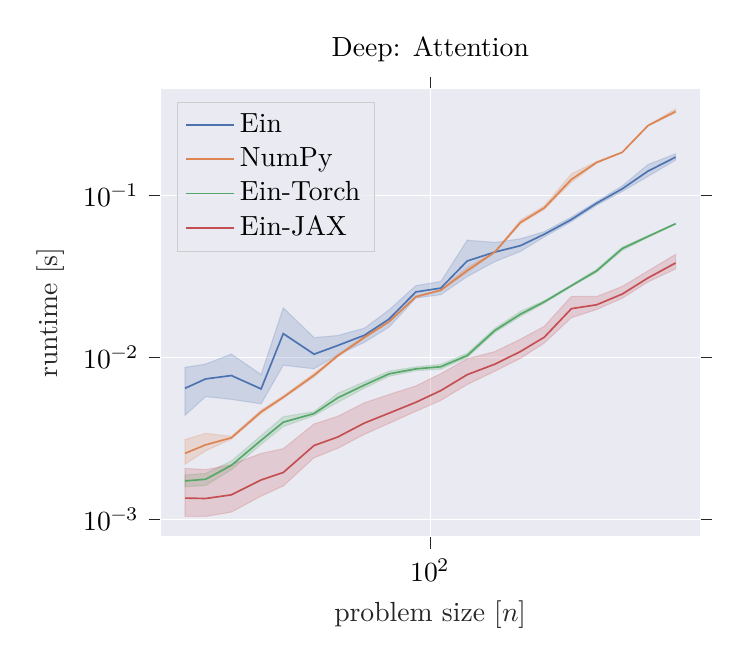
\begin{tikzpicture}

\definecolor{darkslategray38}{RGB}{38,38,38}
\definecolor{indianred1967882}{RGB}{196,78,82}
\definecolor{lavender234234242}{RGB}{234,234,242}
\definecolor{lightgray204}{RGB}{204,204,204}
\definecolor{mediumseagreen85168104}{RGB}{85,168,104}
\definecolor{peru22113282}{RGB}{221,132,82}
\definecolor{steelblue76114176}{RGB}{76,114,176}

\begin{axis}[
axis background/.style={fill=lavender234234242},
axis line style={white},
legend cell align={left},
legend style={
  fill opacity=0.8,
  draw opacity=1,
  text opacity=1,
  at={(0.03,0.97)},
  anchor=north west,
  draw=lightgray204,
  fill=lavender234234242
},
log basis x={10},
log basis y={10},
tick align=outside,
title={Deep: Attention},
x grid style={white},
xlabel=\textcolor{darkslategray38}{problem size \(\displaystyle [n]\)},
xmajorgrids,
xmajorticks=true,
xmin=46.6516495768404, xmax=214.354692507259,
xmode=log,
xtick style={color=darkslategray38},
xtick={1,10,100,1000,10000},
xticklabels={
  \(\displaystyle {10^{0}}\),
  \(\displaystyle {10^{1}}\),
  \(\displaystyle {10^{2}}\),
  \(\displaystyle {10^{3}}\),
  \(\displaystyle {10^{4}}\)
},
y grid style={white},
ylabel=\textcolor{darkslategray38}{runtime \(\displaystyle [\mathrm{s}]\)},
ymajorgrids,
ymajorticks=true,
ymin=0.00077839036959817, ymax=0.457526748594189,
ymode=log,
ytick style={color=darkslategray38},
ytick={1e-05,0.0001,0.001,0.01,0.1,1,10},
yticklabels={
  \(\displaystyle {10^{-5}}\),
  \(\displaystyle {10^{-4}}\),
  \(\displaystyle {10^{-3}}\),
  \(\displaystyle {10^{-2}}\),
  \(\displaystyle {10^{-1}}\),
  \(\displaystyle {10^{0}}\),
  \(\displaystyle {10^{1}}\)
}
]
\path [draw=steelblue76114176, fill=steelblue76114176, opacity=0.2]
(axis cs:50,0.00866516961777961)
--(axis cs:50,0.00437959733370008)
--(axis cs:53,0.00571136703130833)
--(axis cs:57,0.00549411397931181)
--(axis cs:62,0.00515819448823095)
--(axis cs:66,0.00892478528103311)
--(axis cs:72,0.00848875309562573)
--(axis cs:77,0.0103497280768715)
--(axis cs:83,0.0123574961470513)
--(axis cs:89,0.0153537073681036)
--(axis cs:96,0.0232318204215153)
--(axis cs:103,0.0243470966342829)
--(axis cs:111,0.0315116077092898)
--(axis cs:120,0.0389474992522446)
--(axis cs:129,0.0450581238989071)
--(axis cs:138,0.0553997155387656)
--(axis cs:149,0.0689141282858084)
--(axis cs:160,0.0869645879760659)
--(axis cs:172,0.105726904223739)
--(axis cs:185,0.131048314404507)
--(axis cs:200,0.165113660536008)
--(axis cs:200,0.180641041833345)
--(axis cs:200,0.180641041833345)
--(axis cs:185,0.155048844173325)
--(axis cs:172,0.114410946255666)
--(axis cs:160,0.0916533128799529)
--(axis cs:149,0.0734081268089115)
--(axis cs:138,0.0597020637572213)
--(axis cs:129,0.0539203415942211)
--(axis cs:120,0.0511957639434513)
--(axis cs:111,0.0529041254961703)
--(axis cs:103,0.0293612358650353)
--(axis cs:96,0.0277204202753455)
--(axis cs:89,0.019608219791935)
--(axis cs:83,0.0151259833710719)
--(axis cs:77,0.013628377620571)
--(axis cs:72,0.0132266213948424)
--(axis cs:66,0.020198493437565)
--(axis cs:62,0.007824812572253)
--(axis cs:57,0.0104621480692003)
--(axis cs:53,0.00908270323507167)
--(axis cs:50,0.00866516961777961)
--cycle;

\path [draw=peru22113282, fill=peru22113282, opacity=0.2]
(axis cs:50,0.00310353585159311)
--(axis cs:50,0.00218444558344713)
--(axis cs:53,0.00264099351667625)
--(axis cs:57,0.00312796367951597)
--(axis cs:62,0.00448941067160709)
--(axis cs:66,0.00557242847517711)
--(axis cs:72,0.00755672795249632)
--(axis cs:77,0.0100570621815171)
--(axis cs:83,0.0130532579372449)
--(axis cs:89,0.0164422829610364)
--(axis cs:96,0.0233506864421977)
--(axis cs:103,0.0257494977775032)
--(axis cs:111,0.033438777893418)
--(axis cs:120,0.0445056615972135)
--(axis cs:129,0.0666900751281689)
--(axis cs:138,0.0820565367084694)
--(axis cs:149,0.120457840584569)
--(axis cs:160,0.158036874815908)
--(axis cs:172,0.183906026934872)
--(axis cs:185,0.268949629911049)
--(axis cs:200,0.323277702575238)
--(axis cs:200,0.342407206869608)
--(axis cs:200,0.342407206869608)
--(axis cs:185,0.270939681069608)
--(axis cs:172,0.184995948976445)
--(axis cs:160,0.161979947460587)
--(axis cs:149,0.135785860485587)
--(axis cs:138,0.0860758318697544)
--(axis cs:129,0.0703926157974764)
--(axis cs:120,0.044865218588711)
--(axis cs:111,0.0359047128432406)
--(axis cs:103,0.0261409336381674)
--(axis cs:96,0.02392734355242)
--(axis cs:89,0.0167713351898807)
--(axis cs:83,0.0135379774516235)
--(axis cs:77,0.0103985540208683)
--(axis cs:72,0.00795292652835976)
--(axis cs:66,0.0057852893105983)
--(axis cs:62,0.00471289860325527)
--(axis cs:57,0.00324922433031861)
--(axis cs:53,0.00338942967117329)
--(axis cs:50,0.00310353585159311)
--cycle;

\path [draw=mediumseagreen85168104, fill=mediumseagreen85168104, opacity=0.2]
(axis cs:50,0.00187290531822601)
--(axis cs:50,0.00158513726851878)
--(axis cs:53,0.0016137860001219)
--(axis cs:57,0.00201893411013274)
--(axis cs:62,0.00289776546878525)
--(axis cs:66,0.00373102859269551)
--(axis cs:72,0.0043638359677626)
--(axis cs:77,0.00526634859471565)
--(axis cs:83,0.00644555344442868)
--(axis cs:89,0.00762556502617976)
--(axis cs:96,0.00826393439470511)
--(axis cs:103,0.00844199800456072)
--(axis cs:111,0.00998340065959914)
--(axis cs:120,0.0142332090726544)
--(axis cs:129,0.0178838018784524)
--(axis cs:138,0.0216053634271237)
--(axis cs:149,0.0273835782945794)
--(axis cs:160,0.0335230086783611)
--(axis cs:172,0.0457188929081333)
--(axis cs:185,0.055095821991904)
--(axis cs:200,0.0664708835104172)
--(axis cs:200,0.0671842281804)
--(axis cs:200,0.0671842281804)
--(axis cs:185,0.056459320917976)
--(axis cs:172,0.0479695519078791)
--(axis cs:160,0.0349625464752244)
--(axis cs:149,0.0280033654203467)
--(axis cs:138,0.0224041123807414)
--(axis cs:129,0.0192028373828745)
--(axis cs:120,0.0151070856808665)
--(axis cs:111,0.0105863185380748)
--(axis cs:103,0.00903352225843227)
--(axis cs:96,0.00872550573906673)
--(axis cs:89,0.00820928155905056)
--(axis cs:83,0.0070573557732735)
--(axis cs:77,0.00598837103111767)
--(axis cs:72,0.00462060092172372)
--(axis cs:66,0.00429114082115338)
--(axis cs:62,0.00328256745105565)
--(axis cs:57,0.00228848670919722)
--(axis cs:53,0.00191788660218393)
--(axis cs:50,0.00187290531822601)
--cycle;

\path [draw=indianred1967882, fill=indianred1967882, opacity=0.2]
(axis cs:50,0.00205881323224707)
--(axis cs:50,0.00104124689899113)
--(axis cs:53,0.0010400903012386)
--(axis cs:57,0.00110539173312424)
--(axis cs:62,0.00138889518446576)
--(axis cs:66,0.0016029928755513)
--(axis cs:72,0.00239549333605125)
--(axis cs:77,0.00274089793460654)
--(axis cs:83,0.003342213045646)
--(axis cs:89,0.00390773333814443)
--(axis cs:96,0.00463540845530101)
--(axis cs:103,0.00541510976137866)
--(axis cs:111,0.00678948703619883)
--(axis cs:120,0.00820162525218169)
--(axis cs:129,0.00984654562840018)
--(axis cs:138,0.0122467687309224)
--(axis cs:149,0.0175595193414461)
--(axis cs:160,0.0197309056472951)
--(axis cs:172,0.0231411516457184)
--(axis cs:185,0.0292151280773551)
--(axis cs:200,0.0351284628291287)
--(axis cs:200,0.0431678517648125)
--(axis cs:200,0.0431678517648125)
--(axis cs:185,0.0341627500656422)
--(axis cs:172,0.027380149367324)
--(axis cs:160,0.0237241203101732)
--(axis cs:149,0.0237959453089162)
--(axis cs:138,0.0155229372777814)
--(axis cs:129,0.0129405168089087)
--(axis cs:120,0.0108386296032014)
--(axis cs:111,0.0097959206418152)
--(axis cs:103,0.00792431511245824)
--(axis cs:96,0.00665502165672111)
--(axis cs:89,0.00588912678058672)
--(axis cs:83,0.0052340604459715)
--(axis cs:77,0.00432033834046546)
--(axis cs:72,0.00386931112517196)
--(axis cs:66,0.00272614762906446)
--(axis cs:62,0.00254660686450554)
--(axis cs:57,0.0021701492825976)
--(axis cs:53,0.00202190131528866)
--(axis cs:50,0.00205881323224707)
--cycle;

\addplot [semithick, steelblue76114176]
table {%
50 0.00643274999965797
53 0.00735101454993128
57 0.00771308540133759
62 0.00637658750201808
66 0.0140010272487416
72 0.0104482082519098
77 0.0118259001006663
83 0.0136795625010564
89 0.0172192685517075
96 0.0253301624994492
103 0.0267429874998925
111 0.0393433604527672
120 0.0446574875495571
129 0.0488993959479558
138 0.0575560601129028
149 0.0709554693312384
160 0.0894417500858253
172 0.109759966698766
185 0.141206109501582
200 0.172337763833639
};
\addlegendentry{Ein}
\addplot [semithick, peru22113282]
table {%
50 0.00255128515533029
53 0.0028795089613461
57 0.00318148329340343
62 0.00460141695582579
66 0.00566110787079768
72 0.00774117495072384
77 0.0102194417204102
83 0.0132789852982531
89 0.0165945225562473
96 0.0236534559910623
103 0.025940232301479
111 0.0343576448007313
120 0.0446880515076771
129 0.067997123383816
138 0.0837056615370571
149 0.125628829068229
160 0.159758864971689
172 0.184506074572662
185 0.269923098852367
200 0.32982686899833
};
\addlegendentry{NumPy}
\addplot [semithick, mediumseagreen85168104]
table {%
50 0.00172237945965705
53 0.00176415987976747
57 0.00214939264385376
62 0.00307004820947768
66 0.00397105576327044
72 0.00449107211043373
77 0.00561494950886657
83 0.00673614917752436
89 0.00790025604297564
96 0.00848050888403911
103 0.0087393636749908
111 0.0102517985659017
120 0.0146336277735162
129 0.0184530670706201
138 0.0219870518770367
149 0.0276830294999428
160 0.0341652543630178
172 0.0469080397933075
185 0.0557453297948299
200 0.0668298867097816
};
\addlegendentry{Ein-Torch}
\addplot [semithick, indianred1967882]
table {%
50 0.00134965422105551
53 0.0013415680448473
57 0.00141344694199765
62 0.00174696667797057
66 0.00194345548314172
72 0.00285092328542987
77 0.0032179174217509
83 0.00392467615481708
89 0.0045173176434051
96 0.00527181917109779
103 0.00622426011225447
111 0.00781238090470423
120 0.00906573866683564
129 0.0108542434016427
138 0.0133068508364409
149 0.0199720156130728
160 0.0210991645836497
172 0.0245697380430599
185 0.0309027223601388
200 0.0382407308824617
};
\addlegendentry{Ein-JAX}
\end{axis}

\end{tikzpicture}

% This file was created with tikzplotlib v0.10.1.
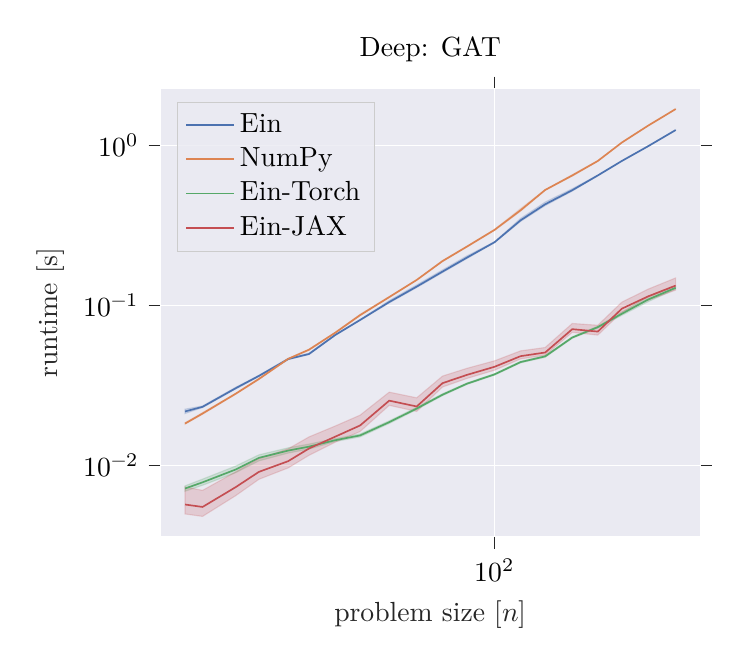
\begin{tikzpicture}

\definecolor{darkslategray38}{RGB}{38,38,38}
\definecolor{indianred1967882}{RGB}{196,78,82}
\definecolor{lavender234234242}{RGB}{234,234,242}
\definecolor{lightgray204}{RGB}{204,204,204}
\definecolor{mediumseagreen85168104}{RGB}{85,168,104}
\definecolor{peru22113282}{RGB}{221,132,82}
\definecolor{steelblue76114176}{RGB}{76,114,176}

\begin{axis}[
axis background/.style={fill=lavender234234242},
axis line style={white},
legend cell align={left},
legend style={
  fill opacity=0.8,
  draw opacity=1,
  text opacity=1,
  at={(0.03,0.97)},
  anchor=north west,
  draw=lightgray204,
  fill=lavender234234242
},
log basis x={10},
log basis y={10},
tick align=outside,
title={Deep: GAT},
x grid style={white},
xlabel=\textcolor{darkslategray38}{problem size \(\displaystyle [n]\)},
xmajorgrids,
xmajorticks=true,
xmin=47.327541132008, xmax=158.470096282431,
xmode=log,
xtick style={color=darkslategray38},
xtick={1,10,100,1000,10000},
xticklabels={
  \(\displaystyle {10^{0}}\),
  \(\displaystyle {10^{1}}\),
  \(\displaystyle {10^{2}}\),
  \(\displaystyle {10^{3}}\),
  \(\displaystyle {10^{4}}\)
},
y grid style={white},
ylabel=\textcolor{darkslategray38}{runtime \(\displaystyle [\mathrm{s}]\)},
ymajorgrids,
ymajorticks=true,
ymin=0.00357140451188423, ymax=2.26106159776395,
ymode=log,
ytick style={color=darkslategray38},
ytick={0.0001,0.001,0.01,0.1,1,10,100},
yticklabels={
  \(\displaystyle {10^{-4}}\),
  \(\displaystyle {10^{-3}}\),
  \(\displaystyle {10^{-2}}\),
  \(\displaystyle {10^{-1}}\),
  \(\displaystyle {10^{0}}\),
  \(\displaystyle {10^{1}}\),
  \(\displaystyle {10^{2}}\)
}
]
\path [draw=steelblue76114176, fill=steelblue76114176, opacity=0.2]
(axis cs:50,0.0224064104077843)
--(axis cs:50,0.0210412454555808)
--(axis cs:52,0.0229158697547246)
--(axis cs:56,0.0299149832124385)
--(axis cs:59,0.0358376364599826)
--(axis cs:63,0.0456729108822037)
--(axis cs:66,0.0491684852679646)
--(axis cs:70,0.0646785691614014)
--(axis cs:74,0.0803627570432022)
--(axis cs:79,0.103316506038318)
--(axis cs:84,0.128890981930363)
--(axis cs:89,0.159859436452669)
--(axis cs:94,0.195611296211367)
--(axis cs:100,0.246378408599412)
--(axis cs:106,0.333690374798607)
--(axis cs:112,0.41918990839913)
--(axis cs:119,0.516446224800893)
--(axis cs:126,0.64382335820701)
--(axis cs:133,0.794372391194338)
--(axis cs:141,0.981472824997036)
--(axis cs:150,1.23903302499966)
--(axis cs:150,1.24767705000122)
--(axis cs:150,1.24767705000122)
--(axis cs:141,0.987544958601939)
--(axis cs:133,0.800509074598085)
--(axis cs:126,0.64970140819787)
--(axis cs:119,0.534673908003606)
--(axis cs:112,0.440913625000394)
--(axis cs:106,0.348489816399524)
--(axis cs:100,0.249056608401588)
--(axis cs:94,0.203338528161112)
--(axis cs:89,0.166099075831049)
--(axis cs:84,0.133873198001311)
--(axis cs:79,0.106884058438336)
--(axis cs:74,0.0812587877306774)
--(axis cs:70,0.0657299229210821)
--(axis cs:66,0.0501189256020007)
--(axis cs:63,0.0465664724373346)
--(axis cs:59,0.0365034048300004)
--(axis cs:56,0.0306932388946916)
--(axis cs:52,0.0234602749724218)
--(axis cs:50,0.0224064104077843)
--cycle;

\path [draw=peru22113282, fill=peru22113282, opacity=0.2]
(axis cs:50,0.0184446637488246)
--(axis cs:50,0.0180389303494724)
--(axis cs:52,0.0208063706469779)
--(axis cs:56,0.027785318992844)
--(axis cs:59,0.0343131169008965)
--(axis cs:63,0.0460556466785556)
--(axis cs:66,0.0523332022301264)
--(axis cs:70,0.0669414899752905)
--(axis cs:74,0.0859334319641273)
--(axis cs:79,0.111642439610493)
--(axis cs:84,0.143552917215477)
--(axis cs:89,0.187321973106492)
--(axis cs:94,0.231179429897902)
--(axis cs:100,0.293751603926884)
--(axis cs:106,0.386191019495534)
--(axis cs:112,0.523593463389857)
--(axis cs:119,0.640901830344275)
--(axis cs:126,0.794109153360786)
--(axis cs:133,1.03776265251244)
--(axis cs:141,1.32023781367195)
--(axis cs:150,1.67623644593477)
--(axis cs:150,1.68644699609881)
--(axis cs:150,1.68644699609881)
--(axis cs:141,1.32596844847007)
--(axis cs:133,1.04090713381635)
--(axis cs:126,0.799377051096404)
--(axis cs:119,0.653990563834111)
--(axis cs:112,0.526348537227738)
--(axis cs:106,0.401894903748126)
--(axis cs:100,0.297173655463371)
--(axis cs:94,0.233740213749402)
--(axis cs:89,0.190098517411969)
--(axis cs:84,0.144045956168409)
--(axis cs:79,0.11321181335858)
--(axis cs:74,0.0877056620071769)
--(axis cs:70,0.0677325927020697)
--(axis cs:66,0.0530688906948059)
--(axis cs:63,0.0464273294289722)
--(axis cs:59,0.0348896895115116)
--(axis cs:56,0.0281341879859182)
--(axis cs:52,0.0213262885845254)
--(axis cs:50,0.0184446637488246)
--cycle;

\path [draw=mediumseagreen85168104, fill=mediumseagreen85168104, opacity=0.2]
(axis cs:50,0.00743295871048535)
--(axis cs:50,0.00687200388019871)
--(axis cs:52,0.0074930098752942)
--(axis cs:56,0.00897587326713843)
--(axis cs:59,0.0106428847682784)
--(axis cs:63,0.0119085282911349)
--(axis cs:66,0.0126129485285033)
--(axis cs:70,0.0140595800550794)
--(axis cs:74,0.0150293664085469)
--(axis cs:79,0.0182432389176254)
--(axis cs:84,0.0222616800430254)
--(axis cs:89,0.0272269726960217)
--(axis cs:94,0.0319773777120358)
--(axis cs:100,0.0365829273842013)
--(axis cs:106,0.0436282533725329)
--(axis cs:112,0.047242670973237)
--(axis cs:119,0.0621273175736479)
--(axis cs:126,0.0719567266462061)
--(axis cs:133,0.0865027543115848)
--(axis cs:141,0.105024522007452)
--(axis cs:150,0.126176274210953)
--(axis cs:150,0.130420841712754)
--(axis cs:150,0.130420841712754)
--(axis cs:141,0.113464524100065)
--(axis cs:133,0.0904368666775504)
--(axis cs:126,0.073952481209692)
--(axis cs:119,0.0634411171924257)
--(axis cs:112,0.0485145711111044)
--(axis cs:106,0.0446024222239718)
--(axis cs:100,0.0373581716624065)
--(axis cs:94,0.0326587859305207)
--(axis cs:89,0.0279756185996088)
--(axis cs:84,0.0230142008905059)
--(axis cs:79,0.0189408876615551)
--(axis cs:74,0.0156786140643163)
--(axis cs:70,0.0146691434408907)
--(axis cs:66,0.0135612458835837)
--(axis cs:63,0.0128472674165502)
--(axis cs:59,0.0116173681917336)
--(axis cs:56,0.00988141689946825)
--(axis cs:52,0.00818949443835985)
--(axis cs:50,0.00743295871048535)
--cycle;

\path [draw=indianred1967882, fill=indianred1967882, opacity=0.2]
(axis cs:50,0.00731889193440033)
--(axis cs:50,0.00495874899108899)
--(axis cs:52,0.00478827120602207)
--(axis cs:56,0.00644950759050617)
--(axis cs:59,0.00816689320752591)
--(axis cs:63,0.00962187027855653)
--(axis cs:66,0.0115327729351214)
--(axis cs:70,0.0139326398565619)
--(axis cs:74,0.0162365970744979)
--(axis cs:79,0.0236683298817417)
--(axis cs:84,0.0216872680642368)
--(axis cs:89,0.0308136652889306)
--(axis cs:94,0.0348492028240012)
--(axis cs:100,0.0392587054763064)
--(axis cs:106,0.0461627059877419)
--(axis cs:112,0.0487399533457126)
--(axis cs:119,0.0676435583134491)
--(axis cs:126,0.0650237155558534)
--(axis cs:133,0.0905544287291479)
--(axis cs:141,0.107433061663371)
--(axis cs:150,0.124204772754486)
--(axis cs:150,0.147991329348705)
--(axis cs:150,0.147991329348705)
--(axis cs:141,0.125908877168537)
--(axis cs:133,0.104513053144372)
--(axis cs:126,0.0749493139939688)
--(axis cs:119,0.0768664639600017)
--(axis cs:112,0.0544041973221155)
--(axis cs:106,0.0518374017672409)
--(axis cs:100,0.0449336621239608)
--(axis cs:94,0.0403161100861066)
--(axis cs:89,0.0360645335703938)
--(axis cs:84,0.0263720795233649)
--(axis cs:79,0.0286191008722177)
--(axis cs:74,0.0205508808193658)
--(axis cs:70,0.0175855829868509)
--(axis cs:66,0.0150278903494274)
--(axis cs:63,0.0126684991309)
--(axis cs:59,0.0110030724841527)
--(axis cs:56,0.00908455295077054)
--(axis cs:52,0.00696318723015097)
--(axis cs:50,0.00731889193440033)
--cycle;

\addplot [semithick, steelblue76114176]
table {%
50 0.0216760998991958
52 0.0231662792510178
56 0.0302682354493299
59 0.0361598061506811
63 0.0460759415494977
66 0.0495460314006777
70 0.0651565495018076
74 0.0808198366900727
79 0.104625850000593
84 0.130679302250428
89 0.16215188114854
94 0.198401333494985
100 0.247568916800083
106 0.33913195799978
112 0.427241775000584
119 0.523064891403192
126 0.64678057480196
133 0.79727589119575
141 0.984185700197122
150 1.2426766582008
};
\addlegendentry{Ein}
\addplot [semithick, peru22113282]
table {%
50 0.0182130364523043
52 0.0210364735598855
56 0.0279562927596381
59 0.03460015871306
63 0.0462338385518484
66 0.0526965015366717
70 0.0673173190473749
74 0.0866866368311044
79 0.112365184951298
84 0.143799225384102
89 0.188661039833064
94 0.232386050729092
100 0.295726299667496
106 0.392010738506597
112 0.524969192960174
119 0.646691693017161
126 0.796551988781993
133 1.03934860479822
141 1.32297764797611
150 1.68100227928949
};
\addlegendentry{NumPy}
\addplot [semithick, mediumseagreen85168104]
table {%
50 0.00715292066259177
52 0.00781948498840287
56 0.00939947963225524
59 0.0111208254302579
63 0.0123486733880478
66 0.0130629380760076
70 0.0143331227714161
74 0.015357040848465
79 0.0185846830770869
84 0.0226133333008199
89 0.0275805378776561
94 0.032319371216476
100 0.0369736208737475
106 0.0441079508953219
112 0.0478854620460647
119 0.0628114840339826
126 0.0729227797616792
133 0.0884276606554327
141 0.108415097274186
150 0.12845207085672
};
\addlegendentry{Ein-Torch}
\addplot [semithick, indianred1967882]
table {%
50 0.00568068419057727
52 0.0054860035885484
56 0.00729115811799732
59 0.00909071010385364
63 0.0106026201235609
66 0.0127219582809245
70 0.0150839495721233
74 0.0177233758812232
79 0.0253218013106487
84 0.0232849760647165
89 0.0325735358667949
94 0.0366899236671074
100 0.0412307227256109
106 0.0480314079229481
112 0.0506300543985476
119 0.0708419455383009
126 0.0684180482507702
133 0.0951441087412742
141 0.113442764289238
150 0.132628757479829
};
\addlegendentry{Ein-JAX}
\end{axis}

\end{tikzpicture}

\end{center}
\begin{center}
% This file was created with tikzplotlib v0.10.1.
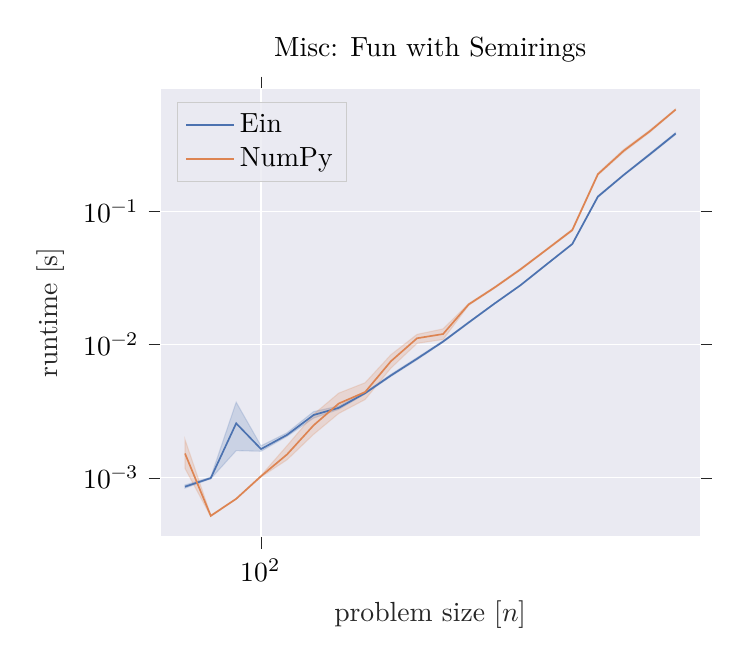
\begin{tikzpicture}

\definecolor{darkslategray38}{RGB}{38,38,38}
\definecolor{lavender234234242}{RGB}{234,234,242}
\definecolor{lightgray204}{RGB}{204,204,204}
\definecolor{peru22113282}{RGB}{221,132,82}
\definecolor{steelblue76114176}{RGB}{76,114,176}

\begin{axis}[
axis background/.style={fill=lavender234234242},
axis line style={white},
legend cell align={left},
legend style={
  fill opacity=0.8,
  draw opacity=1,
  text opacity=1,
  at={(0.03,0.97)},
  anchor=north west,
  draw=lightgray204,
  fill=lavender234234242
},
log basis x={10},
log basis y={10},
tick align=outside,
title={Misc: Fun with Semirings},
x grid style={white},
xlabel=\textcolor{darkslategray38}{problem size \(\displaystyle [n]\)},
xmajorgrids,
xmajorticks=true,
xmin=62.3875656693622, xmax=785.412918011374,
xmode=log,
xtick style={color=darkslategray38},
xtick={1,10,100,1000,10000},
xticklabels={
  \(\displaystyle {10^{0}}\),
  \(\displaystyle {10^{1}}\),
  \(\displaystyle {10^{2}}\),
  \(\displaystyle {10^{3}}\),
  \(\displaystyle {10^{4}}\)
},
y grid style={white},
ylabel=\textcolor{darkslategray38}{runtime \(\displaystyle [\mathrm{s}]\)},
ymajorgrids,
ymajorticks=true,
ymin=0.000360273084941951, ymax=0.840756866074562,
ymode=log,
ytick style={color=darkslategray38},
ytick={1e-05,0.0001,0.001,0.01,0.1,1,10},
yticklabels={
  \(\displaystyle {10^{-5}}\),
  \(\displaystyle {10^{-4}}\),
  \(\displaystyle {10^{-3}}\),
  \(\displaystyle {10^{-2}}\),
  \(\displaystyle {10^{-1}}\),
  \(\displaystyle {10^{0}}\),
  \(\displaystyle {10^{1}}\)
}
]
\path [draw=steelblue76114176, fill=steelblue76114176, opacity=0.2]
(axis cs:70,0.000882980736569152)
--(axis cs:70,0.000836469603709702)
--(axis cs:79,0.000983666491465556)
--(axis cs:89,0.00160017079695535)
--(axis cs:100,0.00158288053147771)
--(axis cs:113,0.00204948378828703)
--(axis cs:128,0.00280844490238451)
--(axis cs:144,0.00326712702590157)
--(axis cs:163,0.00426672655372386)
--(axis cs:184,0.00577486806374509)
--(axis cs:208,0.00770885239919153)
--(axis cs:235,0.0104360073216048)
--(axis cs:265,0.0145424592601194)
--(axis cs:299,0.0201871005468638)
--(axis cs:338,0.0277885871910621)
--(axis cs:381,0.0395295096395785)
--(axis cs:431,0.0567088302808366)
--(axis cs:486,0.127795878605548)
--(axis cs:549,0.187310844089916)
--(axis cs:620,0.264747474796604)
--(axis cs:700,0.379321700398577)
--(axis cs:700,0.392475692002336)
--(axis cs:700,0.392475692002336)
--(axis cs:620,0.273306374798995)
--(axis cs:549,0.190437548428054)
--(axis cs:486,0.131277720707976)
--(axis cs:431,0.0574690455018653)
--(axis cs:381,0.0400586240080884)
--(axis cs:338,0.0281631004092378)
--(axis cs:299,0.0204711578140632)
--(axis cs:265,0.0148268214958807)
--(axis cs:235,0.0106902608964265)
--(axis cs:208,0.00799688121056533)
--(axis cs:184,0.00599107745618312)
--(axis cs:163,0.0043952521038409)
--(axis cs:144,0.00346288692931921)
--(axis cs:128,0.00314344688005804)
--(axis cs:113,0.00217874632706298)
--(axis cs:100,0.00173873103536607)
--(axis cs:89,0.00369602308688627)
--(axis cs:79,0.00101039469656826)
--(axis cs:70,0.000882980736569152)
--cycle;

\path [draw=peru22113282, fill=peru22113282, opacity=0.2]
(axis cs:70,0.00193848101255118)
--(axis cs:70,0.00117677244190284)
--(axis cs:79,0.000512536126241976)
--(axis cs:89,0.000691374327275463)
--(axis cs:100,0.00101480922461673)
--(axis cs:113,0.0013658054360003)
--(axis cs:128,0.00212054063949876)
--(axis cs:144,0.00304233388874813)
--(axis cs:163,0.00387155986232424)
--(axis cs:184,0.00667547516394288)
--(axis cs:208,0.0102306443561746)
--(axis cs:235,0.0109339212095422)
--(axis cs:265,0.019764288904906)
--(axis cs:299,0.0264826368818243)
--(axis cs:338,0.0363230633929786)
--(axis cs:381,0.0508596943735536)
--(axis cs:431,0.0714440472078674)
--(axis cs:486,0.187855203689419)
--(axis cs:549,0.280232980105275)
--(axis cs:620,0.393550276078777)
--(axis cs:700,0.577770442721567)
--(axis cs:700,0.590986770138042)
--(axis cs:700,0.590986770138042)
--(axis cs:620,0.408690926201109)
--(axis cs:549,0.293886953764823)
--(axis cs:486,0.194362045148285)
--(axis cs:431,0.0738519055358364)
--(axis cs:381,0.0519194425429355)
--(axis cs:338,0.0373699798928444)
--(axis cs:299,0.0271283243346789)
--(axis cs:265,0.020363228674962)
--(axis cs:235,0.0131407148729523)
--(axis cs:208,0.0119519829952601)
--(axis cs:184,0.00840683975339437)
--(axis cs:163,0.00517817608230361)
--(axis cs:144,0.00432445873980756)
--(axis cs:128,0.00299782580115713)
--(axis cs:113,0.00174265249451506)
--(axis cs:100,0.00104073359240367)
--(axis cs:89,0.000698650182437273)
--(axis cs:79,0.000523782635826371)
--(axis cs:70,0.00193848101255118)
--cycle;

\addplot [semithick, steelblue76114176]
table {%
70 0.000857760399958352
79 0.000994293649273459
89 0.00256512295018183
100 0.00164436434788513
113 0.00210113954890403
128 0.00296312304708408
144 0.00335419795010239
163 0.00432160414857208
184 0.00587280215040664
208 0.0078401249491435
235 0.0105500666497392
265 0.0146726103506808
299 0.0203304040995135
338 0.027970593853388
381 0.0397933979991649
431 0.0570397616684204
486 0.129457755250769
549 0.188722222330398
620 0.269026924797799
700 0.38559165839979
};
\addlegendentry{Ein}
\addplot [semithick, peru22113282]
table {%
70 0.00152205276548332
79 0.000517646586514327
89 0.000694967112294748
100 0.00102787029947846
113 0.00149808545271352
128 0.00247987456241484
144 0.00361289884685628
163 0.00440781469366663
184 0.00751455303028802
208 0.0111746290230265
235 0.0120248630362191
265 0.020062592361727
299 0.0268113644896092
338 0.0368154788839337
381 0.0513946486001272
431 0.0726436004298779
486 0.190808159953479
549 0.286831809215619
620 0.401049157632001
700 0.583262162683683
};
\addlegendentry{NumPy}
\end{axis}

\end{tikzpicture}

% This file was created with tikzplotlib v0.10.1.
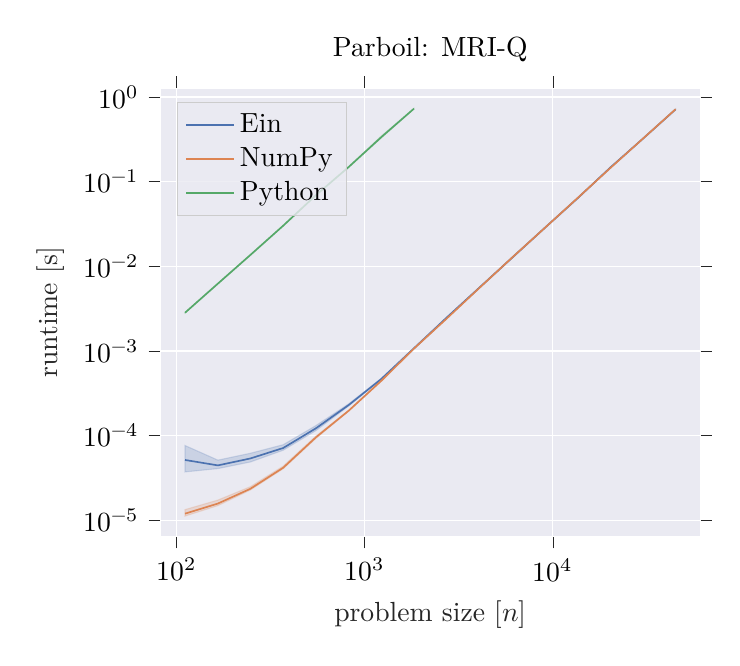
\begin{tikzpicture}

\definecolor{darkslategray38}{RGB}{38,38,38}
\definecolor{lavender234234242}{RGB}{234,234,242}
\definecolor{lightgray204}{RGB}{204,204,204}
\definecolor{mediumseagreen85168104}{RGB}{85,168,104}
\definecolor{peru22113282}{RGB}{221,132,82}
\definecolor{steelblue76114176}{RGB}{76,114,176}

\begin{axis}[
axis background/.style={fill=lavender234234242},
axis line style={white},
legend cell align={left},
legend style={
  fill opacity=0.8,
  draw opacity=1,
  text opacity=1,
  at={(0.03,0.97)},
  anchor=north west,
  draw=lightgray204,
  fill=lavender234234242
},
log basis x={10},
log basis y={10},
tick align=outside,
title={Parboil: MRI-Q},
x grid style={white},
xlabel=\textcolor{darkslategray38}{problem size \(\displaystyle [n]\)},
xmajorgrids,
xmajorticks=true,
xmin=82.2173119053552, xmax=60656.4224057923,
xmode=log,
xtick style={color=darkslategray38},
xtick={1,10,100,1000,10000,100000,1000000},
xticklabels={
  \(\displaystyle {10^{0}}\),
  \(\displaystyle {10^{1}}\),
  \(\displaystyle {10^{2}}\),
  \(\displaystyle {10^{3}}\),
  \(\displaystyle {10^{4}}\),
  \(\displaystyle {10^{5}}\),
  \(\displaystyle {10^{6}}\)
},
y grid style={white},
ylabel=\textcolor{darkslategray38}{runtime \(\displaystyle [\mathrm{s}]\)},
ymajorgrids,
ymajorticks=true,
ymin=6.44509514937527e-06, ymax=1.27001142277489,
ymode=log,
ytick style={color=darkslategray38},
ytick={1e-07,1e-06,1e-05,0.0001,0.001,0.01,0.1,1,10,100},
yticklabels={
  \(\displaystyle {10^{-7}}\),
  \(\displaystyle {10^{-6}}\),
  \(\displaystyle {10^{-5}}\),
  \(\displaystyle {10^{-4}}\),
  \(\displaystyle {10^{-3}}\),
  \(\displaystyle {10^{-2}}\),
  \(\displaystyle {10^{-1}}\),
  \(\displaystyle {10^{0}}\),
  \(\displaystyle {10^{1}}\),
  \(\displaystyle {10^{2}}\)
}
]
\path [draw=steelblue76114176, fill=steelblue76114176, opacity=0.2]
(axis cs:111,7.64748115580005e-05)
--(axis cs:111,3.72972208060673e-05)
--(axis cs:166,4.0835252875695e-05)
--(axis cs:247,4.88473840596271e-05)
--(axis cs:369,6.7268329221406e-05)
--(axis cs:551,0.000114852847618749)
--(axis cs:822,0.000223653940593067)
--(axis cs:1227,0.000462866237739945)
--(axis cs:1830,0.00106242175335865)
--(axis cs:2731,0.00245355305976773)
--(axis cs:4074,0.00557270789158792)
--(axis cs:6078,0.0125523086427165)
--(axis cs:9069,0.0283365872718605)
--(axis cs:13530,0.0632754475533375)
--(axis cs:20185,0.145936900787482)
--(axis cs:30115,0.320605041601812)
--(axis cs:44928,0.712623358200653)
--(axis cs:44928,0.714020192003227)
--(axis cs:44928,0.714020192003227)
--(axis cs:30115,0.321693008599686)
--(axis cs:20185,0.14665374558499)
--(axis cs:13530,0.0637399425110971)
--(axis cs:9069,0.0285860408108601)
--(axis cs:6078,0.0127089362215156)
--(axis cs:4074,0.00564107549882465)
--(axis cs:2731,0.00251207519948366)
--(axis cs:1830,0.00109240443509407)
--(axis cs:1227,0.000473713477222191)
--(axis cs:822,0.000237093156229093)
--(axis cs:551,0.000131444422586355)
--(axis cs:369,7.81547400038107e-05)
--(axis cs:247,6.19402840311523e-05)
--(axis cs:166,5.13782398957119e-05)
--(axis cs:111,7.64748115580005e-05)
--cycle;

\path [draw=peru22113282, fill=peru22113282, opacity=0.2]
(axis cs:111,1.33739018919205e-05)
--(axis cs:111,1.12173942238236e-05)
--(axis cs:166,1.49132007232064e-05)
--(axis cs:247,2.28202668057949e-05)
--(axis cs:369,4.062789333185e-05)
--(axis cs:551,9.28342900732395e-05)
--(axis cs:822,0.000195022538156002)
--(axis cs:1227,0.000440077011060149)
--(axis cs:1830,0.00105853735348736)
--(axis cs:2731,0.00240892100099761)
--(axis cs:4074,0.00553731830009614)
--(axis cs:6078,0.012528845465293)
--(axis cs:9069,0.0282633957795509)
--(axis cs:13530,0.0633936064423404)
--(axis cs:20185,0.143992453522449)
--(axis cs:30115,0.32144269773129)
--(axis cs:44928,0.713192287989754)
--(axis cs:44928,0.720010642417622)
--(axis cs:44928,0.720010642417622)
--(axis cs:30115,0.322048080552488)
--(axis cs:20185,0.144803723048071)
--(axis cs:13530,0.0644441558384659)
--(axis cs:9069,0.0286264725029522)
--(axis cs:6078,0.0128897941919057)
--(axis cs:4074,0.00559594220218362)
--(axis cs:2731,0.00242732959793209)
--(axis cs:1830,0.00108295461147436)
--(axis cs:1227,0.000450903698156903)
--(axis cs:822,0.000199314085446513)
--(axis cs:551,9.87969676543967e-05)
--(axis cs:369,4.36825888719407e-05)
--(axis cs:247,2.49443589484715e-05)
--(axis cs:166,1.73521935363702e-05)
--(axis cs:111,1.33739018919205e-05)
--cycle;

\path [draw=mediumseagreen85168104, fill=mediumseagreen85168104, opacity=0.2]
(axis cs:111,0.00284139199984255)
--(axis cs:111,0.00281315856921844)
--(axis cs:166,0.00620528220835487)
--(axis cs:247,0.0135245814389517)
--(axis cs:369,0.0300064772016471)
--(axis cs:551,0.0690009891442962)
--(axis cs:822,0.148020185515479)
--(axis cs:1227,0.328925585642)
--(axis cs:1830,0.727446436590146)
--(axis cs:1830,0.729701060447134)
--(axis cs:1830,0.729701060447134)
--(axis cs:1227,0.346346094633531)
--(axis cs:822,0.14927478996866)
--(axis cs:551,0.0694211350693412)
--(axis cs:369,0.0302894853075574)
--(axis cs:247,0.0136903077843667)
--(axis cs:166,0.00628679223794377)
--(axis cs:111,0.00284139199984255)
--cycle;

\addplot [semithick, steelblue76114176]
table {%
111 5.16250009241048e-05
166 4.45396020950284e-05
247 5.37770007213112e-05
369 7.14415997208562e-05
551 0.00012215835013194
822 0.000229739699716447
1227 0.000467931201274041
1830 0.00107539789896691
2731 0.00248072924878215
4074 0.00560521049992531
6078 0.0126218833531311
9069 0.0284476669010473
13530 0.0635063490017274
20185 0.146266012140716
30115 0.321243258399772
44928 0.713352350203786
};
\addlegendentry{Ein}
\addplot [semithick, peru22113282]
table {%
111 1.19852447942259e-05
166 1.57818105550113e-05
247 2.35852213674601e-05
369 4.17824449198122e-05
551 9.55665661751828e-05
822 0.000196775694192413
1227 0.000445184290021028
1830 0.00107005975987052
2731 0.00241792426754517
4074 0.00556451805312463
6078 0.0126745723357563
9069 0.0284252734792757
13530 0.0638591521675768
20185 0.144395721890358
30115 0.321745246758947
44928 0.716419132342862
};
\addlegendentry{NumPy}
\addplot [semithick, mediumseagreen85168104]
table {%
111 0.00282732900447953
166 0.00624331846538919
247 0.0136108447615918
369 0.0301533647669631
551 0.0692055784849342
822 0.148659283175515
1227 0.335733234812183
1830 0.728610696513374
};
\addlegendentry{Python}
\end{axis}

\end{tikzpicture}

\end{center}
\begin{center}
% This file was created with tikzplotlib v0.10.1.
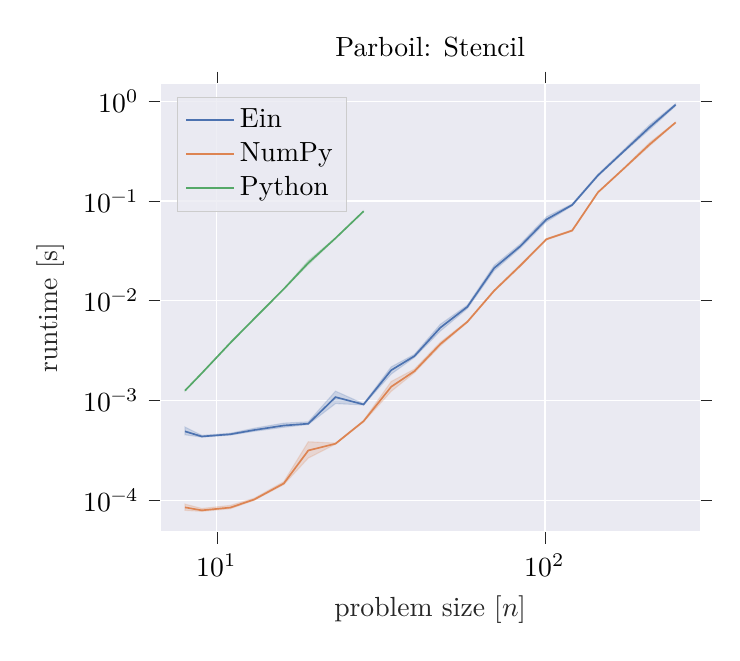
\begin{tikzpicture}

\definecolor{darkslategray38}{RGB}{38,38,38}
\definecolor{lavender234234242}{RGB}{234,234,242}
\definecolor{lightgray204}{RGB}{204,204,204}
\definecolor{mediumseagreen85168104}{RGB}{85,168,104}
\definecolor{peru22113282}{RGB}{221,132,82}
\definecolor{steelblue76114176}{RGB}{76,114,176}

\begin{axis}[
axis background/.style={fill=lavender234234242},
axis line style={white},
legend cell align={left},
legend style={
  fill opacity=0.8,
  draw opacity=1,
  text opacity=1,
  at={(0.03,0.97)},
  anchor=north west,
  draw=lightgray204,
  fill=lavender234234242
},
log basis x={10},
log basis y={10},
tick align=outside,
title={Parboil: Stencil},
x grid style={white},
xlabel=\textcolor{darkslategray38}{problem size \(\displaystyle [n]\)},
xmajorgrids,
xmajorticks=true,
xmin=6.73515331060639, xmax=296.949439421139,
xmode=log,
xtick style={color=darkslategray38},
xtick={0.1,1,10,100,1000,10000},
xticklabels={
  \(\displaystyle {10^{-1}}\),
  \(\displaystyle {10^{0}}\),
  \(\displaystyle {10^{1}}\),
  \(\displaystyle {10^{2}}\),
  \(\displaystyle {10^{3}}\),
  \(\displaystyle {10^{4}}\)
},
y grid style={white},
ylabel=\textcolor{darkslategray38}{runtime \(\displaystyle [\mathrm{s}]\)},
ymajorgrids,
ymajorticks=true,
ymin=4.83051032061226e-05, ymax=1.51304214299554,
ymode=log,
ytick style={color=darkslategray38},
ytick={1e-06,1e-05,0.0001,0.001,0.01,0.1,1,10,100},
yticklabels={
  \(\displaystyle {10^{-6}}\),
  \(\displaystyle {10^{-5}}\),
  \(\displaystyle {10^{-4}}\),
  \(\displaystyle {10^{-3}}\),
  \(\displaystyle {10^{-2}}\),
  \(\displaystyle {10^{-1}}\),
  \(\displaystyle {10^{0}}\),
  \(\displaystyle {10^{1}}\),
  \(\displaystyle {10^{2}}\)
}
]
\path [draw=steelblue76114176, fill=steelblue76114176, opacity=0.2]
(axis cs:8,0.000541935047749575)
--(axis cs:8,0.000453067858434224)
--(axis cs:9,0.000429355900341761)
--(axis cs:11,0.000449767605587112)
--(axis cs:13,0.000491204320896941)
--(axis cs:16,0.000538839243417897)
--(axis cs:19,0.000574791597191506)
--(axis cs:23,0.000931360130489338)
--(axis cs:28,0.000902584986779402)
--(axis cs:34,0.00184224452015769)
--(axis cs:40,0.00270429013589819)
--(axis cs:48,0.00497561136766308)
--(axis cs:58,0.0083633242857286)
--(axis cs:70,0.0200854641618207)
--(axis cs:84,0.0336955659928026)
--(axis cs:101,0.0620397576999039)
--(axis cs:121,0.0895633316013779)
--(axis cs:145,0.177699520667375)
--(axis cs:174,0.309677375195315)
--(axis cs:208,0.519359374797205)
--(axis cs:250,0.901571849806351)
--(axis cs:250,0.945134991791565)
--(axis cs:250,0.945134991791565)
--(axis cs:208,0.578511466801865)
--(axis cs:174,0.328275911873352)
--(axis cs:145,0.185667826333277)
--(axis cs:121,0.0935580004773576)
--(axis cs:101,0.0694506404745198)
--(axis cs:84,0.03691085733215)
--(axis cs:70,0.0226090456772181)
--(axis cs:58,0.00903003433808408)
--(axis cs:48,0.00581493507243067)
--(axis cs:40,0.00289911827871038)
--(axis cs:34,0.00217413936628873)
--(axis cs:28,0.00092799956431918)
--(axis cs:23,0.00124031511919384)
--(axis cs:19,0.000610801349448593)
--(axis cs:16,0.000592792265306343)
--(axis cs:13,0.000526802544554812)
--(axis cs:11,0.000469785337154463)
--(axis cs:9,0.000446724885805452)
--(axis cs:8,0.000541935047749575)
--cycle;

\path [draw=peru22113282, fill=peru22113282, opacity=0.2]
(axis cs:8,9.13596512038154e-05)
--(axis cs:8,7.91657086267016e-05)
--(axis cs:9,7.73303893172656e-05)
--(axis cs:11,8.21614088033308e-05)
--(axis cs:13,9.99987730910563e-05)
--(axis cs:16,0.000143655783890312)
--(axis cs:19,0.000264574498680686)
--(axis cs:23,0.000365250698994858)
--(axis cs:28,0.000610801170047995)
--(axis cs:34,0.00123471806723196)
--(axis cs:40,0.00189975958156038)
--(axis cs:48,0.00353642528071143)
--(axis cs:58,0.00606321318274284)
--(axis cs:70,0.0124189869511541)
--(axis cs:84,0.0219762063405069)
--(axis cs:101,0.0407717955827718)
--(axis cs:121,0.0498527350103243)
--(axis cs:145,0.120981924009612)
--(axis cs:174,0.210022050049381)
--(axis cs:208,0.355438718990264)
--(axis cs:250,0.609366626672306)
--(axis cs:250,0.61736012092859)
--(axis cs:250,0.61736012092859)
--(axis cs:208,0.38465304082684)
--(axis cs:174,0.215096195849646)
--(axis cs:145,0.123596176361213)
--(axis cs:121,0.0513678632191388)
--(axis cs:101,0.0420714220593185)
--(axis cs:84,0.023028867715002)
--(axis cs:70,0.0128413578502985)
--(axis cs:58,0.00625039350995157)
--(axis cs:48,0.0038478141557566)
--(axis cs:40,0.00206198302403562)
--(axis cs:34,0.0015508935681735)
--(axis cs:28,0.000631648145628399)
--(axis cs:23,0.000374060347589935)
--(axis cs:19,0.000385554545724589)
--(axis cs:16,0.000153494512630142)
--(axis cs:13,0.000104623943702111)
--(axis cs:11,8.87077325713449e-05)
--(axis cs:9,8.26492469642159e-05)
--(axis cs:8,9.13596512038154e-05)
--cycle;

\path [draw=mediumseagreen85168104, fill=mediumseagreen85168104, opacity=0.2]
(axis cs:8,0.0012659812533587)
--(axis cs:8,0.00124678293925191)
--(axis cs:9,0.00186972866893111)
--(axis cs:11,0.00375912878122672)
--(axis cs:13,0.00657057378940949)
--(axis cs:16,0.0130797217000369)
--(axis cs:19,0.0230161577127175)
--(axis cs:23,0.0422440562527591)
--(axis cs:28,0.078720046293707)
--(axis cs:28,0.0792059575627619)
--(axis cs:28,0.0792059575627619)
--(axis cs:23,0.0427538768824543)
--(axis cs:19,0.0252667824897221)
--(axis cs:16,0.0131840415997233)
--(axis cs:13,0.00665563404754166)
--(axis cs:11,0.00382769138591117)
--(axis cs:9,0.00188651765983936)
--(axis cs:8,0.0012659812533587)
--cycle;

\addplot [semithick, steelblue76114176]
table {%
8 0.000490091650135582
9 0.00043558534962358
11 0.000458699947921559
13 0.00050575009881868
16 0.000561285449657589
19 0.0005851313493622
23 0.00108082085134811
28 0.000912118700216524
34 0.00201392704766477
40 0.00278657515082159
48 0.00538161674849107
58 0.00869469794924953
70 0.0212869855029567
84 0.0351202103032847
101 0.0653614270631806
121 0.0913993370909752
145 0.181004548501126
174 0.316765899996972
208 0.546782341599464
250 0.923486833198695
};
\addlegendentry{Ein}
\addplot [semithick, peru22113282]
table {%
8 8.47601791404994e-05
9 7.91695351916375e-05
11 8.44630429538325e-05
13 0.000101679819065032
16 0.000147276848182292
19 0.000315438086191837
23 0.000368938222948831
28 0.000619920396183299
34 0.00137503175349805
40 0.00196653281810455
48 0.00368448892433253
58 0.00615190295006863
70 0.0126113480173802
84 0.0224496099670639
101 0.041402507229599
121 0.0505987697507714
145 0.122319606508964
174 0.212361871103318
208 0.368015794918882
250 0.613350352027503
};
\addlegendentry{NumPy}
\addplot [semithick, mediumseagreen85168104]
table {%
8 0.00125621954094339
9 0.00187764126625355
11 0.00379152600667076
13 0.00661218941234588
16 0.0131311919068916
19 0.023976585210625
23 0.0424380686665551
28 0.0789373184016279
};
\addlegendentry{Python}
\end{axis}

\end{tikzpicture}

% This file was created with tikzplotlib v0.10.1.
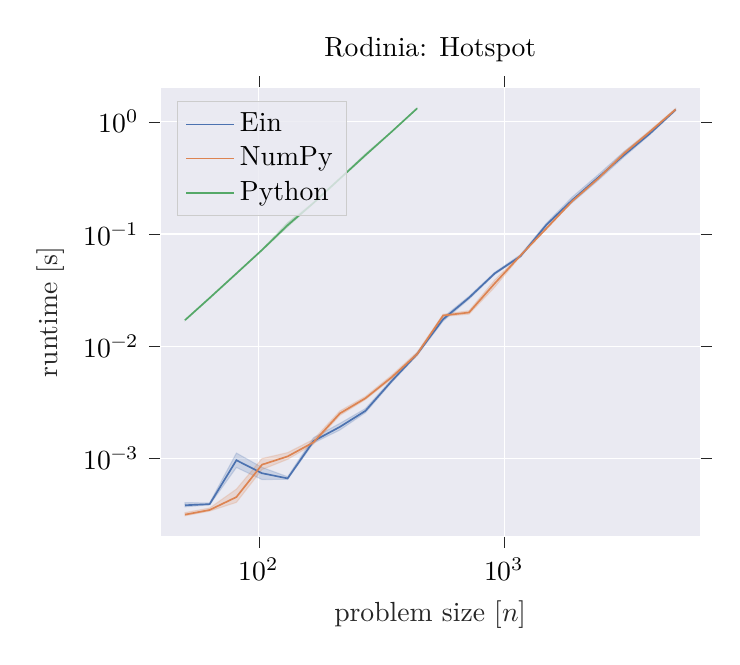
\begin{tikzpicture}

\definecolor{darkslategray38}{RGB}{38,38,38}
\definecolor{lavender234234242}{RGB}{234,234,242}
\definecolor{lightgray204}{RGB}{204,204,204}
\definecolor{mediumseagreen85168104}{RGB}{85,168,104}
\definecolor{peru22113282}{RGB}{221,132,82}
\definecolor{steelblue76114176}{RGB}{76,114,176}

\begin{axis}[
axis background/.style={fill=lavender234234242},
axis line style={white},
legend cell align={left},
legend style={
  fill opacity=0.8,
  draw opacity=1,
  text opacity=1,
  at={(0.03,0.97)},
  anchor=north west,
  draw=lightgray204,
  fill=lavender234234242
},
log basis x={10},
log basis y={10},
tick align=outside,
title={Rodinia: Hotspot},
x grid style={white},
xlabel=\textcolor{darkslategray38}{problem size \(\displaystyle [n]\)},
xmajorgrids,
xmajorticks=true,
xmin=39.7164117362141, xmax=6294.62705897084,
xmode=log,
xtick style={color=darkslategray38},
xtick={1,10,100,1000,10000,100000},
xticklabels={
  \(\displaystyle {10^{0}}\),
  \(\displaystyle {10^{1}}\),
  \(\displaystyle {10^{2}}\),
  \(\displaystyle {10^{3}}\),
  \(\displaystyle {10^{4}}\),
  \(\displaystyle {10^{5}}\)
},
y grid style={white},
ylabel=\textcolor{darkslategray38}{runtime \(\displaystyle [\mathrm{s}]\)},
ymajorgrids,
ymajorticks=true,
ymin=0.000201498092592216, ymax=2.00986678493088,
ymode=log,
ytick style={color=darkslategray38},
ytick={1e-05,0.0001,0.001,0.01,0.1,1,10,100},
yticklabels={
  \(\displaystyle {10^{-5}}\),
  \(\displaystyle {10^{-4}}\),
  \(\displaystyle {10^{-3}}\),
  \(\displaystyle {10^{-2}}\),
  \(\displaystyle {10^{-1}}\),
  \(\displaystyle {10^{0}}\),
  \(\displaystyle {10^{1}}\),
  \(\displaystyle {10^{2}}\)
}
]
\path [draw=steelblue76114176, fill=steelblue76114176, opacity=0.2]
(axis cs:50,0.00040093945186527)
--(axis cs:50,0.000368074528014404)
--(axis cs:63,0.000383445476672932)
--(axis cs:81,0.000825838538330572)
--(axis cs:103,0.000644772650684899)
--(axis cs:131,0.000647616701608058)
--(axis cs:167,0.00136470559069494)
--(axis cs:214,0.00178437005424712)
--(axis cs:272,0.00254733308358482)
--(axis cs:347,0.00471379582675581)
--(axis cs:442,0.00828688624365895)
--(axis cs:564,0.0167107987225791)
--(axis cs:719,0.0262008863759002)
--(axis cs:916,0.0437042131731141)
--(axis cs:1167,0.0622562896341378)
--(axis cs:1488,0.118060100646188)
--(axis cs:1896,0.190832166402834)
--(axis cs:2416,0.300329749798402)
--(axis cs:3079,0.486450566604617)
--(axis cs:3923,0.76613618300762)
--(axis cs:5000,1.26078589159588)
--(axis cs:5000,1.3012147084024)
--(axis cs:5000,1.3012147084024)
--(axis cs:3923,0.816607733399724)
--(axis cs:3079,0.541300269858912)
--(axis cs:2416,0.337273958601872)
--(axis cs:1896,0.213914475007914)
--(axis cs:1488,0.124943806214368)
--(axis cs:1167,0.0654436717586123)
--(axis cs:916,0.0455387166381115)
--(axis cs:719,0.0278046610032288)
--(axis cs:564,0.0180667039872242)
--(axis cs:442,0.00872899553934985)
--(axis cs:347,0.00499742749540019)
--(axis cs:272,0.00276927246466585)
--(axis cs:214,0.00204196582904842)
--(axis cs:167,0.00152384682147385)
--(axis cs:131,0.000682757289960136)
--(axis cs:103,0.000827624445300898)
--(axis cs:81,0.00111092252625895)
--(axis cs:63,0.000398907133476314)
--(axis cs:50,0.00040093945186527)
--cycle;

\path [draw=peru22113282, fill=peru22113282, opacity=0.2]
(axis cs:50,0.00032673171002542)
--(axis cs:50,0.000306223809256533)
--(axis cs:63,0.000337079613283184)
--(axis cs:81,0.000403104442021472)
--(axis cs:103,0.000791844439091519)
--(axis cs:131,0.000976233270458262)
--(axis cs:167,0.00133326872230646)
--(axis cs:214,0.00240886333381857)
--(axis cs:272,0.003335313129242)
--(axis cs:347,0.00508983559719171)
--(axis cs:442,0.00821648794715782)
--(axis cs:564,0.018363774495602)
--(axis cs:719,0.0192549980784647)
--(axis cs:916,0.0335724327249124)
--(axis cs:1167,0.0636838874629534)
--(axis cs:1488,0.110583235301932)
--(axis cs:1896,0.193861714741803)
--(axis cs:2416,0.306879325940162)
--(axis cs:3079,0.505523018210414)
--(axis cs:3923,0.799800217307046)
--(axis cs:5000,1.264736683983)
--(axis cs:5000,1.31620264555326)
--(axis cs:5000,1.31620264555326)
--(axis cs:3923,0.837685994555397)
--(axis cs:3079,0.539811122722255)
--(axis cs:2416,0.318958040986727)
--(axis cs:1896,0.199532320670354)
--(axis cs:1488,0.114055102252696)
--(axis cs:1167,0.0652174438192701)
--(axis cs:916,0.0388684300518635)
--(axis cs:719,0.0206627060913336)
--(axis cs:564,0.0192027732355738)
--(axis cs:442,0.00883587755718326)
--(axis cs:347,0.00546277709638322)
--(axis cs:272,0.00355156857035007)
--(axis cs:214,0.00263857985262473)
--(axis cs:167,0.00147028904430777)
--(axis cs:131,0.00112115848759694)
--(axis cs:103,0.000992268569379521)
--(axis cs:81,0.000529755718533716)
--(axis cs:63,0.000359117092669337)
--(axis cs:50,0.00032673171002542)
--cycle;

\path [draw=mediumseagreen85168104, fill=mediumseagreen85168104, opacity=0.2]
(axis cs:50,0.0171492615072016)
--(axis cs:50,0.0169266795758594)
--(axis cs:63,0.0266131099362991)
--(axis cs:81,0.0440128870918064)
--(axis cs:103,0.07126383819766)
--(axis cs:131,0.116134618129277)
--(axis cs:167,0.187049734661776)
--(axis cs:214,0.308844255432755)
--(axis cs:272,0.496620497434416)
--(axis cs:347,0.81118520515641)
--(axis cs:442,1.31659624124695)
--(axis cs:442,1.32251089329489)
--(axis cs:442,1.32251089329489)
--(axis cs:347,0.812763998462663)
--(axis cs:272,0.519172390597327)
--(axis cs:214,0.314748820935053)
--(axis cs:167,0.191087127589291)
--(axis cs:131,0.125872881631466)
--(axis cs:103,0.0727092836864279)
--(axis cs:81,0.0447864388573507)
--(axis cs:63,0.0270812682079353)
--(axis cs:50,0.0171492615072016)
--cycle;

\addplot [semithick, steelblue76114176]
table {%
50 0.000380316599330399
63 0.000389060348970816
81 0.000958352151792496
103 0.000733785350894323
131 0.000660091650934191
167 0.00141973749778117
214 0.00190174600284081
272 0.00264312924773549
347 0.00484016244954546
442 0.00849062289998983
564 0.0173506560495298
719 0.0269802436996542
916 0.04452330624772
1167 0.0634414349378858
1488 0.120880361001279
1896 0.200819791603135
2416 0.31828747499967
3079 0.505030508202617
3923 0.783784091603593
5000 1.28100029999914
};
\addlegendentry{Ein}
\addplot [semithick, peru22113282]
table {%
50 0.000313751671644151
63 0.00034511540423769
81 0.000449974981914862
103 0.000874762900493183
131 0.00103676393950919
167 0.00138504208322672
214 0.00250934550967851
272 0.00342247601949238
347 0.00524075549648738
442 0.00849938419192227
564 0.0187414299273627
719 0.0199229283698736
916 0.0362555841655364
1167 0.0644407811628573
1488 0.112207148416363
1896 0.196310843395679
2416 0.312149828431074
3079 0.521080107533942
3923 0.814798008302104
5000 1.28977514403189
};
\addlegendentry{NumPy}
\addplot [semithick, mediumseagreen85168104]
table {%
50 0.0170372362644735
63 0.0268527433421794
81 0.0444024117848814
103 0.0719782158874706
131 0.119667906225472
167 0.189060234167748
214 0.311685812135787
272 0.504449041617114
347 0.812088850100548
442 1.31957545728193
};
\addlegendentry{Python}
\end{axis}

\end{tikzpicture}

\end{center}
\begin{center}
% This file was created with tikzplotlib v0.10.1.
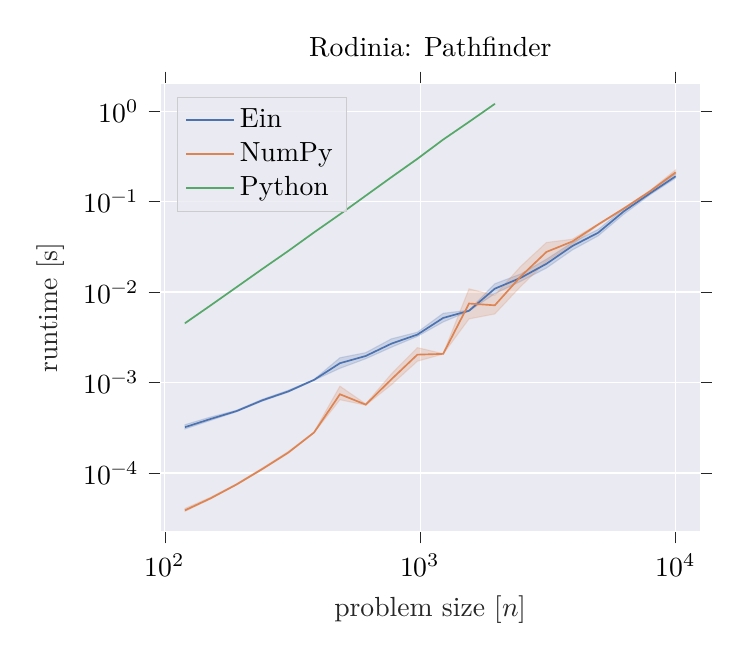
\begin{tikzpicture}

\definecolor{darkslategray38}{RGB}{38,38,38}
\definecolor{lavender234234242}{RGB}{234,234,242}
\definecolor{lightgray204}{RGB}{204,204,204}
\definecolor{mediumseagreen85168104}{RGB}{85,168,104}
\definecolor{peru22113282}{RGB}{221,132,82}
\definecolor{steelblue76114176}{RGB}{76,114,176}

\begin{axis}[
axis background/.style={fill=lavender234234242},
axis line style={white},
legend cell align={left},
legend style={
  fill opacity=0.8,
  draw opacity=1,
  text opacity=1,
  at={(0.03,0.97)},
  anchor=north west,
  draw=lightgray204,
  fill=lavender234234242
},
log basis x={10},
log basis y={10},
tick align=outside,
title={Rodinia: Pathfinder},
x grid style={white},
xlabel=\textcolor{darkslategray38}{problem size \(\displaystyle [n]\)},
xmajorgrids,
xmajorticks=true,
xmin=96.1922998493838, xmax=12475.0110131366,
xmode=log,
xtick style={color=darkslategray38},
xtick={1,10,100,1000,10000,100000,1000000},
xticklabels={
  \(\displaystyle {10^{0}}\),
  \(\displaystyle {10^{1}}\),
  \(\displaystyle {10^{2}}\),
  \(\displaystyle {10^{3}}\),
  \(\displaystyle {10^{4}}\),
  \(\displaystyle {10^{5}}\),
  \(\displaystyle {10^{6}}\)
},
y grid style={white},
ylabel=\textcolor{darkslategray38}{runtime \(\displaystyle [\mathrm{s}]\)},
ymajorgrids,
ymajorticks=true,
ymin=2.2418522596979e-05, ymax=2.02262511777973,
ymode=log,
ytick style={color=darkslategray38},
ytick={1e-06,1e-05,0.0001,0.001,0.01,0.1,1,10,100},
yticklabels={
  \(\displaystyle {10^{-6}}\),
  \(\displaystyle {10^{-5}}\),
  \(\displaystyle {10^{-4}}\),
  \(\displaystyle {10^{-3}}\),
  \(\displaystyle {10^{-2}}\),
  \(\displaystyle {10^{-1}}\),
  \(\displaystyle {10^{0}}\),
  \(\displaystyle {10^{1}}\),
  \(\displaystyle {10^{2}}\)
}
]
\path [draw=steelblue76114176, fill=steelblue76114176, opacity=0.2]
(axis cs:120,0.000341726930964796)
--(axis cs:120,0.000306472893898899)
--(axis cs:151,0.000380524324009457)
--(axis cs:191,0.000475164178642444)
--(axis cs:241,0.000622518288109859)
--(axis cs:304,0.000780791235338256)
--(axis cs:384,0.00105858095441363)
--(axis cs:485,0.0014339613285847)
--(axis cs:612,0.00182949863126851)
--(axis cs:772,0.00245332813254208)
--(axis cs:975,0.00322873239420005)
--(axis cs:1230,0.0046603400319691)
--(axis cs:1553,0.00614925598643822)
--(axis cs:1960,0.0095943368870212)
--(axis cs:2474,0.0131162009411673)
--(axis cs:3122,0.0184126407171061)
--(axis cs:3941,0.0291354026384579)
--(axis cs:4974,0.0417086751744864)
--(axis cs:6277,0.0726598048349842)
--(axis cs:7923,0.118049233426548)
--(axis cs:10000,0.1817131320034)
--(axis cs:10000,0.204999416671247)
--(axis cs:10000,0.204999416671247)
--(axis cs:7923,0.128127749075995)
--(axis cs:6277,0.083734567083649)
--(axis cs:4974,0.0490543335992334)
--(axis cs:3941,0.0353001864768157)
--(axis cs:3122,0.0230370064200542)
--(axis cs:2474,0.0158103541443779)
--(axis cs:1960,0.0123458300823404)
--(axis cs:1553,0.0063026045256629)
--(axis cs:1230,0.00581660559701049)
--(axis cs:975,0.00359588766476008)
--(axis cs:772,0.00303963665832271)
--(axis cs:612,0.00213747135527228)
--(axis cs:485,0.0018773853993298)
--(axis cs:384,0.00108018522152634)
--(axis cs:304,0.000818749898280657)
--(axis cs:241,0.000652531522373465)
--(axis cs:191,0.000493188765976811)
--(axis cs:151,0.000415084914093313)
--(axis cs:120,0.000341726930964796)
--cycle;

\path [draw=peru22113282, fill=peru22113282, opacity=0.2]
(axis cs:120,4.05292028394652e-05)
--(axis cs:120,3.76572221177818e-05)
--(axis cs:151,5.15489040017335e-05)
--(axis cs:191,7.37133692938077e-05)
--(axis cs:241,0.000108863147358759)
--(axis cs:304,0.00016458389057526)
--(axis cs:384,0.000277424925640168)
--(axis cs:485,0.000644754050045128)
--(axis cs:612,0.000561306121472983)
--(axis cs:772,0.000945457267077864)
--(axis cs:975,0.00171881254987961)
--(axis cs:1230,0.00206152069904944)
--(axis cs:1553,0.00504187347480254)
--(axis cs:1960,0.00572239232308683)
--(axis cs:2474,0.0115250413096875)
--(axis cs:3122,0.0217258990204398)
--(axis cs:3941,0.0334428679968257)
--(axis cs:4974,0.0548838507420711)
--(axis cs:6277,0.0824095292239567)
--(axis cs:7923,0.126775335965419)
--(axis cs:10000,0.201898616792484)
--(axis cs:10000,0.224101366947745)
--(axis cs:10000,0.224101366947745)
--(axis cs:7923,0.132007286081162)
--(axis cs:6277,0.0853363105666736)
--(axis cs:4974,0.0565887416299204)
--(axis cs:3941,0.0383505131565081)
--(axis cs:3122,0.03528248513181)
--(axis cs:2474,0.0192043702785523)
--(axis cs:1960,0.00920419509298448)
--(axis cs:1553,0.0108464514986388)
--(axis cs:1230,0.00208173524225237)
--(axis cs:975,0.0024281130370177)
--(axis cs:772,0.00124802802831195)
--(axis cs:612,0.00057954685688131)
--(axis cs:485,0.000910760384406102)
--(axis cs:384,0.000283834486956713)
--(axis cs:304,0.000172147029546981)
--(axis cs:241,0.00011356738586769)
--(axis cs:191,7.60678164252169e-05)
--(axis cs:151,5.38777557057058e-05)
--(axis cs:120,4.05292028394652e-05)
--cycle;

\path [draw=mediumseagreen85168104, fill=mediumseagreen85168104, opacity=0.2]
(axis cs:120,0.00455871063264353)
--(axis cs:120,0.00449157143116792)
--(axis cs:151,0.00705664282240553)
--(axis cs:191,0.0112666225017015)
--(axis cs:241,0.0179427403300778)
--(axis cs:304,0.0282595000777108)
--(axis cs:384,0.045413275318881)
--(axis cs:485,0.0720816022037464)
--(axis cs:612,0.115601016419376)
--(axis cs:772,0.18487746708988)
--(axis cs:975,0.293471200991418)
--(axis cs:1230,0.481217045161424)
--(axis cs:1553,0.755620449817535)
--(axis cs:1960,1.19882571494297)
--(axis cs:1960,1.2041320192535)
--(axis cs:1960,1.2041320192535)
--(axis cs:1553,0.766056252441126)
--(axis cs:1230,0.486687586993213)
--(axis cs:975,0.300764526207406)
--(axis cs:772,0.187704668997105)
--(axis cs:612,0.11655834188607)
--(axis cs:485,0.0725001043405431)
--(axis cs:384,0.0457697327409285)
--(axis cs:304,0.0284581307418256)
--(axis cs:241,0.0180423590589997)
--(axis cs:191,0.011370876864278)
--(axis cs:151,0.00713747732596371)
--(axis cs:120,0.00455871063264353)
--cycle;

\addplot [semithick, steelblue76114176]
table {%
120 0.000320914650365012
151 0.000395139447937254
191 0.000483020901447162
241 0.000635822951153386
304 0.000795981250121258
384 0.00106819585125777
485 0.0016338312496373
612 0.0019634500516986
772 0.00269066685068537
975 0.00338468330010073
1230 0.00516932915124926
1553 0.00620426465029595
1960 0.0108929021487711
2474 0.014341264700488
3122 0.0205118332502025
3941 0.0322111937006412
4974 0.0452253313495021
6277 0.0781504904600577
7923 0.122558375112324
10000 0.19009911116882
};
\addlegendentry{Ein}
\addplot [semithick, peru22113282]
table {%
120 3.86600244931162e-05
151 5.23924914005125e-05
191 7.46212748891676e-05
241 0.000110693301001573
304 0.000167543510974984
384 0.000279794247711953
485 0.000741863875427135
612 0.000569439187306788
772 0.00108637716541252
975 0.0020312529826725
1230 0.00207120530354192
1553 0.00746278985508761
1960 0.00712931676217431
2474 0.0148365315915019
3122 0.0277522884342686
3941 0.0361839926787512
4974 0.0557543046914908
6277 0.0839329969844282
7923 0.129218504613934
10000 0.210188051602755
};
\addlegendentry{NumPy}
\addplot [semithick, mediumseagreen85168104]
table {%
120 0.00452345369735408
151 0.00709796155077178
191 0.0113156319885714
241 0.0179928968837197
304 0.0283531498755143
384 0.0455828779890031
485 0.0722714566850368
612 0.116039105793265
772 0.186124559536344
975 0.296669488554691
1230 0.483990980228694
1553 0.759446551183138
1960 1.20162530253334
};
\addlegendentry{Python}
\end{axis}

\end{tikzpicture}

% This file was created with tikzplotlib v0.10.1.
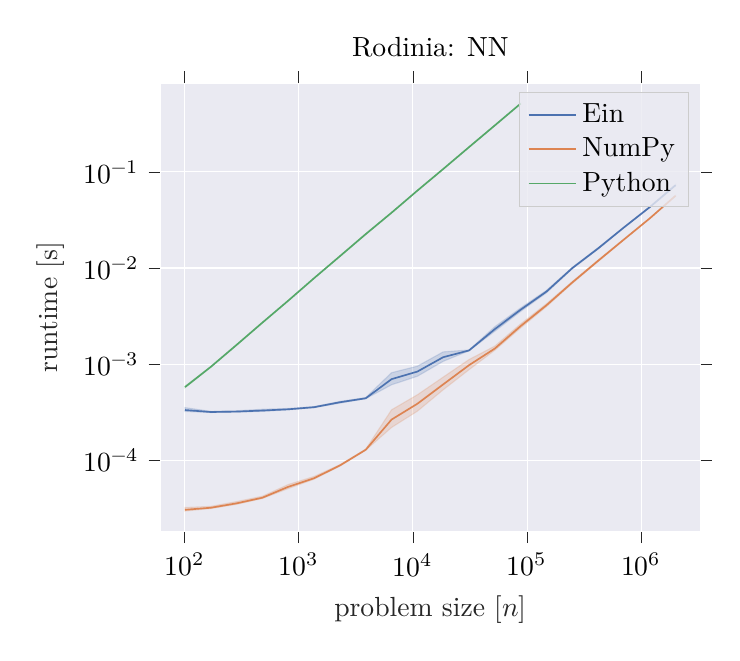
\begin{tikzpicture}

\definecolor{darkslategray38}{RGB}{38,38,38}
\definecolor{lavender234234242}{RGB}{234,234,242}
\definecolor{lightgray204}{RGB}{204,204,204}
\definecolor{mediumseagreen85168104}{RGB}{85,168,104}
\definecolor{peru22113282}{RGB}{221,132,82}
\definecolor{steelblue76114176}{RGB}{76,114,176}

\begin{axis}[
axis background/.style={fill=lavender234234242},
axis line style={white},
legend cell align={left},
legend style={
  fill opacity=0.8,
  draw opacity=1,
  text opacity=1,
  draw=lightgray204,
  fill=lavender234234242
},
log basis x={10},
log basis y={10},
tick align=outside,
title={Rodinia: NN},
x grid style={white},
xlabel=\textcolor{darkslategray38}{problem size \(\displaystyle [n]\)},
xmajorgrids,
xmajorticks=true,
xmin=61.5865594359247, xmax=3279936.43174958,
xmode=log,
xtick style={color=darkslategray38},
xtick={1,10,100,1000,10000,100000,1000000,10000000,100000000},
xticklabels={
  \(\displaystyle {10^{0}}\),
  \(\displaystyle {10^{1}}\),
  \(\displaystyle {10^{2}}\),
  \(\displaystyle {10^{3}}\),
  \(\displaystyle {10^{4}}\),
  \(\displaystyle {10^{5}}\),
  \(\displaystyle {10^{6}}\),
  \(\displaystyle {10^{7}}\),
  \(\displaystyle {10^{8}}\)
},
y grid style={white},
ylabel=\textcolor{darkslategray38}{runtime \(\displaystyle [\mathrm{s}]\)},
ymajorgrids,
ymajorticks=true,
ymin=1.81947944318841e-05, ymax=0.839521688084527,
ymode=log,
ytick style={color=darkslategray38},
ytick={1e-06,1e-05,0.0001,0.001,0.01,0.1,1,10},
yticklabels={
  \(\displaystyle {10^{-6}}\),
  \(\displaystyle {10^{-5}}\),
  \(\displaystyle {10^{-4}}\),
  \(\displaystyle {10^{-3}}\),
  \(\displaystyle {10^{-2}}\),
  \(\displaystyle {10^{-1}}\),
  \(\displaystyle {10^{0}}\),
  \(\displaystyle {10^{1}}\)
}
]
\path [draw=steelblue76114176, fill=steelblue76114176, opacity=0.2]
(axis cs:101,0.000353183350853215)
--(axis cs:101,0.000322000755368208)
--(axis cs:170,0.000314380267118395)
--(axis cs:286,0.000317003530926741)
--(axis cs:481,0.000322697213905485)
--(axis cs:810,0.000334883444993466)
--(axis cs:1364,0.000352830739120691)
--(axis cs:2297,0.000393298693052202)
--(axis cs:3866,0.000437682356459845)
--(axis cs:6508,0.000610060642447934)
--(axis cs:10954,0.000748529692882585)
--(axis cs:18439,0.00107022395513923)
--(axis cs:31037,0.0013778470563193)
--(axis cs:52243,0.00220267150323707)
--(axis cs:87937,0.00354220306126081)
--(axis cs:148018,0.00552566797723557)
--(axis cs:249149,0.00984000897233273)
--(axis cs:419374,0.0157586040781098)
--(axis cs:705902,0.0262687281757098)
--(axis cs:1188194,0.0427564917887139)
--(axis cs:2000000,0.0721616613371225)
--(axis cs:2000000,0.0738775504718173)
--(axis cs:2000000,0.0738775504718173)
--(axis cs:1188194,0.0434651341967401)
--(axis cs:705902,0.0266722735361873)
--(axis cs:419374,0.0162754852996295)
--(axis cs:249149,0.0101439765249415)
--(axis cs:148018,0.00586161805647862)
--(axis cs:87937,0.0038486267659755)
--(axis cs:52243,0.00245423619433495)
--(axis cs:31037,0.00140523523068623)
--(axis cs:18439,0.0013424137828224)
--(axis cs:10954,0.000953390890881565)
--(axis cs:6508,0.000815215431102843)
--(axis cs:3866,0.00044905472001119)
--(axis cs:2297,0.00040965498505102)
--(axis cs:1364,0.000361619109044113)
--(axis cs:810,0.000346027625691931)
--(axis cs:481,0.000339486644388671)
--(axis cs:286,0.000327328193470748)
--(axis cs:170,0.000322710332693532)
--(axis cs:101,0.000353183350853215)
--cycle;

\path [draw=peru22113282, fill=peru22113282, opacity=0.2]
(axis cs:101,3.22559100401596e-05)
--(axis cs:101,2.96449693902489e-05)
--(axis cs:170,3.14934114268439e-05)
--(axis cs:286,3.48214441480291e-05)
--(axis cs:481,4.00659476672678e-05)
--(axis cs:810,5.07766298240826e-05)
--(axis cs:1364,6.35731459038473e-05)
--(axis cs:2297,8.71387222680512e-05)
--(axis cs:3866,0.0001274504644238)
--(axis cs:6508,0.000219516355946705)
--(axis cs:10954,0.00032421837460516)
--(axis cs:18439,0.000541176797972362)
--(axis cs:31037,0.000875860084372431)
--(axis cs:52243,0.00139754218193783)
--(axis cs:87936.9999999999,0.00238507747289486)
--(axis cs:148018,0.00397239848397111)
--(axis cs:249149,0.00693343404896193)
--(axis cs:419374,0.011701289388949)
--(axis cs:705902,0.0196380316798663)
--(axis cs:1188194,0.0327551329863903)
--(axis cs:2000000,0.0563697438910666)
--(axis cs:2000000,0.0567656971331198)
--(axis cs:2000000,0.0567656971331198)
--(axis cs:1188194,0.0330266446635957)
--(axis cs:705902,0.020009598896486)
--(axis cs:419374,0.0121253361396363)
--(axis cs:249149,0.00723793720397841)
--(axis cs:148018,0.00425602114828713)
--(axis cs:87936.9999999999,0.00262417958025749)
--(axis cs:52243,0.00154237070974182)
--(axis cs:31037,0.00111702348559922)
--(axis cs:18439,0.000733776703379504)
--(axis cs:10954,0.000480482764834311)
--(axis cs:6508,0.000334941548718695)
--(axis cs:3866,0.000130604314644266)
--(axis cs:2297,9.00585693711033e-05)
--(axis cs:1364,6.78827531542254e-05)
--(axis cs:810,5.5947379509631e-05)
--(axis cs:481,4.22765473712785e-05)
--(axis cs:286,3.71984245268413e-05)
--(axis cs:170,3.31572100669677e-05)
--(axis cs:101,3.22559100401596e-05)
--cycle;

\path [draw=mediumseagreen85168104, fill=mediumseagreen85168104, opacity=0.2]
(axis cs:101,0.000589457024414009)
--(axis cs:101,0.000568953687788088)
--(axis cs:170,0.000932760601906098)
--(axis cs:286,0.00157676212682705)
--(axis cs:481,0.00269014023387063)
--(axis cs:810,0.00456824403507154)
--(axis cs:1364,0.00781684567576174)
--(axis cs:2297,0.0132332147399879)
--(axis cs:3866,0.0224030687894545)
--(axis cs:6508,0.0375410743138903)
--(axis cs:10954,0.0636976314951003)
--(axis cs:18439,0.106880695886844)
--(axis cs:31037,0.180381141286895)
--(axis cs:52243,0.302955803728834)
--(axis cs:87936.9999999999,0.513305702468478)
--(axis cs:87936.9999999999,0.515261943256742)
--(axis cs:87936.9999999999,0.515261943256742)
--(axis cs:52243,0.306912435547992)
--(axis cs:31037,0.181994994172091)
--(axis cs:18439,0.107544237911094)
--(axis cs:10954,0.0641120078648686)
--(axis cs:6508,0.0377682359528933)
--(axis cs:3866,0.0227212726354391)
--(axis cs:2297,0.0133415728676727)
--(axis cs:1364,0.00787460561231384)
--(axis cs:810,0.00458809586848752)
--(axis cs:481,0.00272029211130062)
--(axis cs:286,0.00159993491855368)
--(axis cs:170,0.000943961562623982)
--(axis cs:101,0.000589457024414009)
--cycle;

\addplot [semithick, steelblue76114176]
table {%
101 0.000333293699804926
170 0.000317854050808819
286 0.000321154150879011
481 0.000329189600597601
810 0.000339143750170479
1364 0.000356783248571446
2297 0.000401624949881807
3866 0.000441795850929338
6508 0.000698466801986797
10954 0.000837535450409632
18439 0.00118185419923975
31037 0.0013890062495193
52243 0.00231618305042502
87937 0.00368823744938709
148018 0.00569290025014197
249149 0.00999016645146185
419374 0.0160098270993331
705902 0.0264645334005763
1188194 0.043052987599367
2000000 0.0728267559284827
};
\addlegendentry{Ein}
\addplot [semithick, peru22113282]
table {%
101 3.05528342139521e-05
170 3.2091806616217e-05
286 3.56759428016795e-05
481 4.08118615742292e-05
810 5.29794457754726e-05
1364 6.50958708510871e-05
2297 8.83896944339121e-05
3866 0.000128688389726388
6508 0.000265278999709473
10954 0.000387513753608334
18439 0.000616376754286184
31037 0.000975915411108311
52243 0.00145488893584056
87936.9999999999 0.00249228061874149
148018 0.00410179624561609
249149 0.00708321676797298
419374 0.0119003698396945
705902 0.0198239321008911
1188194 0.0328866681925195
2000000 0.0565629873357129
};
\addlegendentry{NumPy}
\addplot [semithick, mediumseagreen85168104]
table {%
101 0.000577430156660138
170 0.000938021977295833
286 0.00158729640319589
481 0.00270493801690121
810 0.00457767140090912
1364 0.00784705169005239
2297 0.0132865399300266
3866 0.0225482732543257
6508 0.037647948818945
10954 0.0639124892179613
18439 0.107201755226209
31037 0.181154204295067
52243 0.304895639952628
87936.9999999999 0.514365493283406
};
\addlegendentry{Python}
\end{axis}

\end{tikzpicture}

\end{center}

\chapter{Compiler outputs}

This brief appendix concerns the compiler outputs for a short example program. Intermediate representations in Phi and Yarr are printed using the compiler's debug utilities. For clarity, a hand-written Python program using NumPy which is equivalent to the Yarr code is given.

\section*{Ein}

We use Ein's Python API to implement \textcolor{blue}{\texttt{pairwiseL1}}. Type annotations are applied, and the code is successfully type-checked by \texttt{mypy}.

\begin{center}    
\begin{cminted}{python}
from ein import array, fold, Vec, Int, Float
from typing import Callable

def fold_sum(f: Callable[[Int], Float]) -> Float:
    return fold(wrap(0.0), lambda i, acc: acc + f(i))

def L1(u: Vec[Float], v: Vec[Float]) -> Float:
    return fold_sum(lambda i: abs(u[i] - v[i]))

def pairwiseL1(A: Vec[Vec[Float]]) -> Vec[Vec[Float]]:
    return array(lambda i, j: L1(A[i], A[j]))
\end{cminted}
\end{center}

\section*{Phi}

We construct the Phi term for \texttt{pairwiseL1} via 
\mintinline{python}{ein.function(pairwiseL1).phi(ein.ndarray_type(2, float))}
The term is printed as follows (\texttt{\&x} denote variables, where \texttt{\&0} is the argument \texttt{A}, \texttt{@i} are indices):
\begin{center}
\begin{cminted}{ocaml}
let &1: int = size[0](&0) in
let &2: int = size[1](&0) in
for @0[&1]. 
  for @1[&1]. 
    fold &3[&2] init &4: float = 0.0 by &4 => 
      &4 + (let &5: float = &0[@0][&3] - &0[@1][&3] in
            if less(0.0, &5) then &5 else -&5)
\end{cminted}
\end{center}
To make the example more interesting, the absolute value is computed here via a conditional: 
$$|x| = \mathrm{where}(0 < x, x, -x)$$

\section*{Yarr}

We apply code generation on Phi to obtain Yarr code, which uses primitives similar to NumPy routines.

\begin{center}    
\begin{cminted}{ocaml}
let &6: int = size[1](&0) in
let &7: [][]float = unsqueeze((0, 1), 0.0) in
let &8: [][]float = 
  let &9: int = size[0](&0) in
  repeat(1, &9, repeat(0, &9, &7))
in
fold &3[&6] init &4: [][]float = &8 by &4 => 
  add(&4, 
    let &10: [][]float = 
      let &11: []float = take(&0, None, &3) in
      subtract(unsqueeze((1,), &11), &11)
    in
    where(less(0.0, &10), &10, negative(&10))
  )
\end{cminted}
\end{center}

\section*{NumPy}

I hand-simplified the Yarr output into an equivalent Python program using NumPy directly. 

\begin{center}    
\begin{cminted}{python}
from numpy import *

def pairwiseL1(x0: ndarray) -> ndarray:
    x6, x9 = x0.shape[1]
    x4 = zeros((x6, x9))
    for i in range(x1):
        x11 = x0[:, i]
        x10 = expand_dims(x11, axis=1) - x11
        x4 += where(x10 < 0, x10, -x10)
    return x4
\end{cminted}
\end{center}

  \chapter{Project Proposal}

\newcommand{\dontcite}[1]{}

\textit{The following is quoted verbatim. However, formatting and citations were adjusted to be consistent with the rest of this document.}

\section{Introduction}

Tensors are an ubiquitous abstraction in the area of machine learning. In this context, they are $n$-dimensional arrays specialised for high-performance data parallel computing. The Python programming language dominates the machine learning research scene. However, its runtime overheads are far too high for the data processing to be expressed directly in the language. As such, Python highly benefits from the tensor abstraction with a set of highly optimised operations. This gave rise libraries and frameworks such as NumPy \cite{harris2020array}, PyTorch and TensorFlow.

These aforementioned libraries all share a common core of the \textit{array programming model}, as introduced in APL \cite{iverson1962programming}. The model is characterised by first-class multi-dimensional arrays. Primitives are parameterised in nontrivial ways, acting on the arrays as a whole -- individual elements are rarely referenced. The core benefit of this approach is that the implementations of individual primitives -- referred to as \textit{kernels} -- can be highly optimised (and written in another language). Programs in the model can also be surprisingly concise, as can be seen on Figure \ref{fig:pairwise-l1-numpy}. 

\begin{figure}[h]
    \centering
    \begin{minipage}{0.65\textwidth}
    \begin{minted}{python}
def pairwiseL1(a):
    return sum(abs(a.T - a[..., newaxis]), axis=1) 
    \end{minted}
    \end{minipage}
    \caption{Computing a matrix of pairwise $L_1$ distances between rows with axis manipulation and broadcasting in NumPy -- as given by Dex authors \cite{maclaurin2019dex}}
    \label{fig:pairwise-l1-numpy}
\end{figure}

Despite its widespread use in today's scientific computing and machine learning workflows, the array programming model is not without its problems. The available operations expose features such as broadcasting, which allow high expressiveness without sacrificing performance. However, these features also make programs difficult to write, debug and maintain \cite{paszke2021getting}. They are also nontrivial to statically analyse due to being highly dynamic, as the behaviour of operators may vary based on the shapes and element types of their inputs \dontcite{liu2020type}. This causes the need for comments in the host language, as few facilities exist for type annotations \dontcite{Rush2018}. Additionally, the actual implementation in terms of the available kernels may be distant from the mathematical description of a computation -- as can be seen in Figure \ref{fig:pairwise-l1-math}. The choice of kernels is not obvious, as their number is usually in the hundreds. More involved pieces of logic have to be expressed with more specialised kernels (if they exist), or otherwise complex  combinations of existing ones (suboptimal performance), or worst of all expressed directly in Python, which significantly hurts performance.

\begin{figure}[h]
    \centering
    $$ \texttt{pairwiseL1}(A)_{i,j} = \sum_{k} \left| A_{i,k} - A_{j,k} \right|  $$
    \caption{An index-oriented mathematical formulation of \texttt{pairwiseL1} from Figure \ref{fig:pairwise-l1-numpy}}
    \label{fig:pairwise-l1-math}
\end{figure}

All in all, these shortcomings cause novel deep learning architectures to be unreasonably difficult to express and optimise in the array programming model. This invites the exploration of new array programming paradigms which seek to solve these problems.

Dex \cite{paszke2021getting} is a recent research programming language implementing \textit{pointful} (or \textit{index-oriented}) array programming, which can be seen as a generalisation of \textit{Einstein summation notation}. Its distinctive feature is the \texttt{for} primitive, where an array's elements may be defined in terms of their indices. Programs written with this approach boast closeness to mathematical notation (Figure \ref{fig:pairwise-l1-dex}). Index bounds are inferred as in Einstein summation for clarity. Dependent types fulfil a central role for statically analysing array sizes. Dex demonstrates that the paradigm can achieve performance comparable to other approaches, such as the \textit{array-combinator} language Futhark \cite{henriksen2017futhark}.

\begin{figure}[h]
    \centering
    \begin{minipage}{0.6\textwidth}        
    \begin{minted}{haskell}
def pairwiseL1 (a : m=>n=>Float) : n=>n=>Float =
    for i. for j. sum for k. abs (a.i.k - a.j.k) 
    \end{minted}
    \end{minipage}
    \caption{Computation of \texttt{pairwiseL1} from Figure \ref{fig:pairwise-l1-numpy} in Dex}
    \label{fig:pairwise-l1-dex}
\end{figure}

However, application of an entirely new language like Dex poses further problems, such as its usability in the existing ecosystem. Embedding the DSL \cite{gibbons2014folding} is a popular approach to address this. Jax \cite{frostig2018compiling} can be seen as a domain-specific language within a shallow embedding in Python. Operations performed on Jax arrays are \textit{traced} into a staged expression. That IR can then be e.g. differentiated, and compiled for execution via XLA \dontcite{jax2018github}. This approach is in contrast to the deep embeddings used in TensorFlow and PyTorch, which manipulate the Python AST. Shallow embeddings are generally better composable and more predictable.

\section{Description}

The main goal of the project is to design and implement a pointful array programming domain-specific language in a shallow Python embedding, lending itself to being easy to use, statically analyse, and execute efficiently.

The basis of the DSL would be formed by an underlying calculus -- provisionally named \textit{Ein}~and~\textit{Phi} respectively. Phi could be based on the semantics of Dex. A proposed basic version of this calculus is shown in Figure \ref{fig:phi-calculus}. Its core feature is vector comprehensions -- defining tensors in terms of their elements as functions of indices. It is not an aim for the core language to include all Dex features such as algebraic effects and dependent types, though similar ideas can be developed as extensions. Phi can be extended with more arithmetic functions and reductions (like product).

\begin{figure}[h]
    \centering
    \begin{align*}
        e ::=& \quad \Phi\, i[e].\, e & \text{(vector comprehension)} \\
        |& \quad \Sigma\, i[e].\, e  & \text{(vector summation)} \\
        |& \quad e[e]  & \text{(indexing)} \\
        |& \quad e + e \quad | \quad e \cdot e \quad | \quad e - e \quad | \quad e \mathop{/} e   & \text{(scalar arithmetic)} \\
        |& \quad i \quad | \quad x &\text{(index value, variable)}
    \end{align*} 
    $$ \texttt{pairwiseL1}(a) = \Phi \,i[n].\, \Phi \,j[n].\, \Sigma\, k[m].\,
    \texttt{abs}\left( a[i][k] - a[j][k] \right) $$
    \caption{Proposed structure of the Phi calculus. Below an example term is given, where $a$ has shape $n \times m$. All three variables are given in scope.}
    \label{fig:phi-calculus}
\end{figure}
A computation in Ein should be traced, and then staged for execution by a \textit{backend}. As NumPy is universally available and has good performance on CPU, it is planned to be the primary backend. Hence, a core part of the project is compilation of expressions in the DSL to an efficient sequence of NumPy calls necessary to execute it.

Though Python is the host language, compilation can happen in another language -- for instance Rust, as it interfaces well with Python via PyO3 \dontcite{PyO3} and is better suited for compiler-related tasks with static types and ADTs. I plan to resolve this in early stages of the project.

\begin{figure}[h]
    \centering
    \begin{minted}{python}
n, m = a.shape
# tensor and sum are primitives in Ein, corresponding to phi and sigma in Phi
dist = tensor[n, n](lambda i, j: sum[m](lambda k: abs(a[i, k] - a[j, k])))
# dist may be computed with NumPy arrays:
x = a.reshape(n, 1, m)  # x[i, *j, k] = a[i, k]
y = a.reshape(1, n, m)  # y[*i, j, k] = a[j, k]
z = x - y               # z[i, j, k] = a[i, k] - a[j, k]
w = z.abs()             # w[i, j, k] = abs(a[i, k] - a[j, k])
dist = w.sum(axis=2)    # dist[i, j] = sum(k: abs(a[i, k] - a[j, k]))
\end{minted}
    \caption{Code example in Ein, along with a sequence of NumPy calls for executing it.}
    \label{fig:pairwise-l1-ein}
\end{figure}

\needspace{1em}
\section{Starting point}

I have no experience designing or implementing a machine learning domain-specific language or compiler. I expect the knowledge from Part IB Semantics, Compiler Construction and Concepts courses will be useful during design and development, and that the Part II Denotational Semantics and Types may also be helpful when working on extensions to the semantics and type system of the language. Part IA Scientific Computing and Part IB Data Science gave me an insight into array programming in NumPy itself, though I have also used NumPy in personal projects.

I have been exposed to the domain of machine learning during my open-source work on the ONNX project, which is an industry standard IR for describing models. Working on a research project on Graph Neural Networks during Part IB has also given me some domain experience. I have years of Python experience, including professional, and basic experience with Rust.

Prior to starting the project I had done a fair amount of research into the topic of array programming, including papers on index-oriented techniques and compiler optimisations relevant to linear algebra and machine learning. I had not written any project-specific code before 1~October, though I have written experiments to test the feasibility of some of the ideas.

\section{Goals}

\subsection{Core}

\paragraph{Formalisation} Design and formalise operational semantics of a calculus for expressing pointful array programming. A basic type system (up to tensor element type and rank) to validate these terms should be given. These may be based on a subset of the rules presented in Paszke et al. \cite{paszke2021getting}.

\paragraph{Embedding} Implement a Python API for constructing Phi calculus terms, forming Ein. The terms should be easy to serialise, to make way for tooling developed in other languages.

\paragraph{Execution} Create a NumPy execution backend for evaluating Phi expressions. The computation should be orchestrated into a sequence of necessary calls.

\paragraph{Testing} Collate an Ein test and benchmark suite, based on the ones in Dex and Futhark. Results should be compared to NumPy implementations in terms of correctness and performance.

\subsection{Extensions}

\paragraph{Optimisation} The terms in the calculus benefit from relative expressiveness, and their purity makes them easy to manipulate. Many optimisations could be derived with equality saturation \dontcite{10.14778/3407790.3407799}, for instance as implemented in the egg library \dontcite{2021-egg}. A focus would be on optimisations which are not performed by existing frameworks, for instance in linear algebra \dontcite{9835658}. This may also include loop fusion, finding common subexpressions (up to arrays), and axis ordering.

\paragraph{Backends} Execution with different compatible frameworks in the style of Einops \cite{rogozhnikov2021einops} is a large benefit which allows using the DSL within an existing project -- for instance one employing PyTorch or Jax. These are relatively similar to NumPy, and so the implementation should be as well. In the direction of a classical compiler, implementing C code generation or compiling directly with LLVM is also possible for portability and slightly better performance. Lastly, state-of-the-art deep learning compilers like XLA \dontcite{50530} or TVM \dontcite{10.5555/3291168.3291211} could be used directly.

\paragraph{Types} Dynamic sizes in array types are difficult to design types for. Possible solutions include a unification-based approach with existential types \dontcite{Abe2015ASA}, or Futhark's size-dependent types \cite{henriksen2021towards}. Advanced static analyses could be done with an SMT solver like Z3 \dontcite{2008-z3}. Another direction is basic parametric polymorphism for numeric types in the style of Haskell's \texttt{Num} and \texttt{Floating} typeclasses. 

\paragraph{Further expressiveness} Capabilities like domain-specific intrinsics (e.g. matrix inverse), allowing usage of sequential loops or jagged arrays, and custom reductions (besides summation).

\paragraph{Program transformation} Ranges from basic syntactic sugar for inferring index bounds deriving from Einstein summation, up to automatic differentiation (forward or backward) which may base on the approach in Dex \cite{paszke2021getting} or Jax \cite{frostig2018compiling}. 

\section{Success criteria}

\begin{itemize}
    \item Presenting a design of the Phi pointful array calculus. An integral part is definition of tensors with their elements defined in terms of their indices, as in Dex \cite{paszke2021getting}.
    \item A shallow embedding of the Ein DSL in Python, with an API that constructs Phi calculus terms via tracing. The technique may draw on Jax \cite{frostig2018compiling}.
    \item Implementation of an execution backend for Ein, which compiles the terms into a form that may leverage libraries in the Python ecosystem.
    \item An evaluation of correctness, performance and expressiveness of Ein.
\end{itemize}

\section{Evaluation strategy}


The evaluation would be performed on a test and benchmark suite derived from the ones in existing projects -- such as Dex \cite{paszke2021getting} and Futhark \cite{henriksen2017futhark}. They themselves are based on other existing suites like Parboil \dontcite{Stratton2012ParboilAR}. Other sources of program samples include modern deep learning model architectures, like transformers or graph neural networks.
\paragraph{Correctness} The test suite can be used to demonstrate general correctness of the language. If an execution backend is not trivially derived from the operational semantics, a formal proof of correctness may also be given.

\paragraph{Performance} Performance should be comparable to existing approaches when the code is casually written without additional care given to performance. Reaching state-of-the-art performance is not within the scope of the project.

\paragraph{Expressiveness} Successful creation of a representative test suite will demonstrate the expressiveness of the language. It should be noted that instances of sequential logic (where usage of control flow primitives like algebraic effects in Dex or \texttt{loop} in Futhark is necessary) are considered an extension. This is motivated by their relative rarity in deep learning frameworks, where they are seldom the focus of optimisation.

% \paragraph{Usability} The language should present a higher degree of code readability than in frameworks employing the array programming model on an example in the target domain, such as an implementation of an attention layer (or another one present in the benchmark suite). An absence of axis indexing and self-documenting through index names are considered pluses \cite{Rush_2018}.

\section{Timetable}

\subsection{Michaelmas Term}

\begin{itemize}
    \item \textbf{Weeks 2 -- 4} (October \nth{12} -- November \nth{1})  \begin{itemize}
        \item Review literature on tensor languages and index-oriented approaches, particularly Dex.
        \item Construct the semantics and type system of Phi.
        \item Ensure the type system meets required properties, formulate a Progress theorem.
        \item \textbf{Milestone.} Formal pointful array programming calculus as a basis for Ein.
    \end{itemize}
    \item \textbf{Weeks 5 -- 6} (November \nth{2} -- November \nth{15}) 
 \begin{itemize}
        \item Implement an API for constructing Phi calculus terms.     
        \item Create a fundamental backend for evaluating terms in pure Python without the usage of an array library.
        \item Construct small correctness test cases suitable for the basic backend.
        \item \textbf{Milestone.} Ein embedded in Python with basic evaluation.
    \end{itemize}
    \item \textbf{Weeks 7 -- 8} (November \nth{16} -- November \nth{29}) \begin{itemize}
        \item Design the NumPy execution backend and construct a term evaluation algorithm.
        \item Prove the correctness of term evaluation under reasonable assumptions.
        \item Implement the NumPy staging and execution backend.
        \item \textbf{Milestone.} NumPy execution backend passing basic tests.
    \end{itemize}
\end{itemize}

\subsection{Michaelmas Vacation}

\begin{itemize}
    \item \textbf{Weeks 1 -- 3} (November \nth{30} -- December \nth{20}) \begin{itemize}
        \item Collate a test and benchmark suite from the Futhark, Dex and other codebases.
        \item Based on testing feedback, fix and improve on the NumPy backend.
        \item \textit{Extensions.} Implement syntactic sugar (e.g. bounds inference) to ease writing the suite. 
        \item \textbf{Milestone.} NumPy execution backend tested and effective.
    \end{itemize}

    \item \textbf{Weeks 4 -- 5} (December \nth{21} -- January \nth{3}) -- Break for Christmas.

    \item \textbf{Weeks 6 -- 7} (January \nth{4} -- January \nth{17}) \begin{itemize}
        \item Test, refactor and document the existing code.
        \item Finish and improve any core steps.
        \item Begin work on progress report.
        \item \textbf{Milestone.} \textit{Success criteria met.}
    \end{itemize}
\end{itemize}

\subsection{Lent Term}

\begin{itemize}
    \item \textbf{Weeks 1 -- 2} (January \nth{18} -- January \nth{31})  \begin{itemize}
        \item Write the progress report and start work on slides.
        \item \textit{Extensions.} Preparatory work and determining feasibility. Attempt evaluation of real-world deep learning model within the DSL. Implement support for intrinsics like linear algebra routines.
        \item \textbf{Milestone.} Progress Report [February 2].
    \end{itemize}
    \item \textbf{Weeks 3 -- 4} (February \nth{1} -- February \nth{14})  \begin{itemize}
        \item Prepare slides for presentation.
        \item \textit{Extensions.} Implement and evaluate backends using a deep learning framework (PyTorch/Jax) and another using code generation (C/LLVM)
        \item \textbf{Milestone.} Progress Report Presentation [February \nth{7} -- February \nth{14}].
    \end{itemize}
    \item \textbf{Weeks 5 -- 6} (February \nth{15} -- February \nth{28}) \begin{itemize}
        \item Dissertation -- Write Chapter 1: Introduction \& Chapter 2: Preparation.
        \item \textit{Extensions.} Experiment with optimisations using equality saturation on one of the existing backends.
    \end{itemize}
    \item \textbf{Weeks 7 -- 8} (February \nth{29} -- March \nth{13}) \begin{itemize}
        \item Dissertation -- Write Chapter 3: Implementation.
        \item \textit{Extensions.} Investigate and attempt an approach to size types.
    \end{itemize}
\end{itemize}

\subsection{Easter Vacation}

\begin{itemize}
    \item \textbf{Weeks 1 -- 2} (March \nth{14} -- March \nth{27})  \begin{itemize}
        \item Dissertation -- Write Chapter 4: Evaluation.
        \item \textit{Extensions.} Finalise the scope and implementation.
    \end{itemize}
    \item \textbf{Weeks 3 -- 4} (March \nth{28} -- April \nth{10})  \begin{itemize}
        \item Dissertation -- Write Chapter 5: Conclusions.
        \item Share full draft with supervisor and directors of studies. 
        \item \textbf{Milestone.} Full dissertation draft shared for review.
    \end{itemize}
    \item \textbf{Weeks 5 -- 6} (April \nth{11} -- April \nth{24})  \begin{itemize}
        \item Address review comments for draft.
        \item \textbf{Milestone.} Reviewed dissertation draft.
    \end{itemize}
\end{itemize}

\subsection{Easter Term}

\begin{itemize}
    \item \textbf{Weeks 1 -- 2} (April \nth{25} -- May \nth{8}) \begin{itemize}
        \item Editing and proofreading dissertation.
        \item Updating dissertation with latest results from extensions.
        \item Prepare source code for submission.
        \item \textbf{Submission [May \nth{10}]}
    \end{itemize}
\end{itemize}

\section{Resource declaration}

I will use my personal laptop (2021 MacBook Pro, 14-inch) for developing the project. I accept full responsibility for this machine and I have made contingency plans to protect myself against hardware and/or software failure. GitHub will be used to backup the repository and project notes, and Overleaf will be used for the dissertation itself. These are in addition to backups on my other personal devices. All libraries and packages used will be open-source. As part of extensions, I may make use of an external computing cluster, such as the freely available Google Colab or department resources.


  % \printindex

%TC:endignore
\end{document}
